\subsection{Minkowski's inequality}

Let X be a locally compact space, \(\mu\) a measure on X. In the set of positive numerical functions (finite or not) defined on X, the function \(|\mu|^{*}(f)\) is positive, positively homogeneous, increasing and convex ( \(\S1\) , No.~3, Props. 10, 11 and 12).

PROPOSITION 1. --- For every real number \(p \geqslant 1\) and every pair of positive functions \(f, g\) (finite or not) defined on \(X\) ,

\[
\left(| \mu | ^ {*} ((f + g) ^ {p})\right) ^ {1 / p} \leqslant \left(| \mu | ^ {*} (f ^ {p})\right) ^ {1 / p} + \left(| \mu | ^ {*} (g ^ {p})\right) ^ {1 / p}\tag{1}
\]

(Minkowski's inequality).

The inequality (1) is obvious when one of the terms of the second member is equal to \(+\infty\) . In the contrary case, \(f\) and \(g\) are finite almost everywhere (§2, No.~3, Prop. 7). If \(f_1\) and \(g_1\) are finite positive functions equivalent to \(f\) and \(g\) , respectively, then \(f_1^p\) , \(g_1^p\) and \((f_1 + g_1)^p\) are equivalent to \(f^p\) , \(g^p\) and \((f + g)^p\) , respectively, and since equivalent positive functions have the same upper integral (§2, No.~3, Prop. 6), we are reduced to proving the inequality (1) in the case that \(f\) and \(g\) are everywhere finite; but in this case the inequality is a special case of the general Minkowski inequality proved in Ch. I, No.~2, Prop. 3.

We shall also have occasion to make use of the following elementary inequality: if \(p \geqslant 1\) then, for any numbers \(a \geqslant 0\) , \(b \geqslant 0\) ,

\[
a ^ {p} + b ^ {p} \leqslant (a + b) ^ {p}.\tag{2}
\]

The inequality is obvious if \(a = b = 0\) or if one of the numbers \(a, b\) is \(+\infty\) ; if \(a, b\) are finite and \(a + b > 0\) , it may be written

\[
\left(\frac {a}{a + b}\right) ^ {p} + \left(\frac {b}{a + b}\right) ^ {p} \leqslant 1,
\]

which follows from the fact that

\[
\left(\frac {a}{a + b}\right) ^ {p} \leqslant \frac {a}{a + b}, \quad \left(\frac {b}{a + b}\right) ^ {p} \leqslant \frac {b}{a + b} \quad \text { and } \quad \frac {a}{a + b} + \frac {b}{a + b} = 1.
\]

\subsection{\texorpdfstring{The semi-norms \(\mathbf{N}_p\)}{The semi-norms N sub p}}

In all that follows, F denotes a complete normed vector space (that is, a Banach space) over the field R or the field C; the norm of an element \(z \in F\) will be denoted \(|z|\) . Given a mapping f of a set A into F, we write \(|f|\) for the mapping \(x \mapsto |\mathbf{f}(x)|\) of A into \(R_{+}\) (one must take care to note that \(|f|\) is a numerical function, and not a number).

DEFINITION 1. --- Let X be a locally compact space, \(\mu\) a measure on X. For every mapping f of X into a Banach space F, and for every number p such that \(1 \leqslant p < +\infty\) , we denote by \(\mathrm{N}_p(\mathbf{f}, \mu)\) , or simply \(\mathrm{N}_p(\mathbf{f})\) , the positive number \((\int^* |\mathbf{f}|^p d|\mu|)^{1/p}\) .

Note that the number \(N_{p}(\mathbf{f})\) may be equal to \(+\infty\) .

PROPOSITION 2. --- If f and g are two mappings of X into F, and \(\alpha\) is any scalar \(\neq 0\) , then, for \(1 \leqslant p < +\infty\) ,

\begin{enumerate}
\def\labelenumi{(\arabic{enumi})}
\setcounter{enumi}{2}
\tightlist
\item
\end{enumerate}

\[
\mathrm{N} _ {p} (\alpha \mathbf {f}) = | \alpha | \mathrm{N} _ {p} (\mathbf {f})\tag{4}
\]

\[
\mathrm{N} _ {p} (\mathbf {f} + \mathbf {g}) \leqslant \mathrm{N} _ {p} (\mathbf {f}) + \mathrm{N} _ {p} (\mathbf {g}).
\]

For, the relation (3) follows at once from Def. 1 and the fact that \(|\mu|^*\) is positively homogeneous; on the other hand, since \(|\mathbf{f} + \mathbf{g}| \leqslant |\mathbf{f}| + |\mathbf{g}|\) , the inequality (4) follows from Minkowski's inequality (1) and the fact that \(|\mu|^*\) is increasing.

We extend Def. 1 to the case of numerical functions, finite or not, defined on X, by again setting

\[
\mathrm{N} _ {p} (f) = \left(\int^ {*} | f | ^ {p} d | \mu |\right) ^ {1 / p}
\]

for such a function \(f\) . One sees immediately that the relations (3) and (4) also hold for these functions when \(f + g\) is defined on \(X\) and \(\alpha \neq 0\) . Moreover:

THEOREM 1 (countable convexity theorem). --- Let \((f_n)\) be a sequence of functions \(\geqslant 0\) (finite or not) defined on X. For \(1 \leqslant p < +\infty\) ,

\[
\mathrm{N} _ {p} \left(\sum_ {n = 1} ^ {\infty} f _ {n}\right) \leqslant \sum_ {n = 1} ^ {\infty} \mathrm{N} _ {p} (f _ {n}).\tag{5}
\]

Set \(f = \sum_{n=1}^{\infty} f_n\) ; \(f\) is the upper envelope of the increasing sequence of functions \(g_n = \sum_{k=1}^{n} f_k\) ; the definition of \(N sub p(f)\) , and Th. 3 of §1, No.~3, show that \(\mathrm{N}_{p}(f)=\sup_{n}\mathrm{N}_{p}(g_{n})\) . But \(\mathrm{N}_{p}(g_{n})\leqslant\sum_{k=1}^{n}\mathrm{N}_{p}(f_{k})\) by Prop. 1, whence the inequality (5).

PROPOSITION 3. --- If \(\mathbf{f}\) and \(\mathbf{g}\) are two equivalent mappings of X into a Banach space F, then \(\mathrm{N}_p(\mathbf{f} - \mathbf{g}) = 0\) for \(1 \leqslant p < +\infty\) ; conversely, if \(\mathrm{N}_p(\mathbf{f} - \mathbf{g}) = 0\) for a value of \(p \geqslant 1\) then \(\mathbf{f}\) and \(\mathbf{g}\) are equivalent. The proposition follows at once from Th. 1 of §2, No.~3.

If \(\mathbf{f}\) and \(\mathbf{g}\) are two equivalent mappings of \(X\) into \(F\) , then \(\mathrm{N}_p(\mathbf{f}) = \mathrm{N}_p(\mathbf{g})\) for all \(p \geqslant 1\) ( \(\S 2\) , No.~3, Prop. 6); thus, \(\mathrm{N}_p(\mathbf{f})\) depends only on the class \(\widetilde{\mathbf{f}}\) of \(\mathbf{f}\) , and one sets, by definition, \(\mathrm{N}_p(\widetilde{\mathbf{f}}) = \mathrm{N}_p(\mathbf{f})\) . Since the classes of mappings of \(X\) into \(F\) form a vector space ( \(\S 2\) , No.~4), the relations (3) and (4) may also be written

\begin{enumerate}
\def\labelenumi{(\arabic{enumi})}
\setcounter{enumi}{5}
\tightlist
\item
\end{enumerate}

\[
\mathrm{N} _ {p} (\alpha \widetilde {\mathbf {f}}) = | \alpha | \mathrm{N} _ {p} (\widetilde {\mathbf {f}})\tag{7}
\]

\[
\mathrm{N} _ {p} (\widetilde {\mathbf {f}} + \widetilde {\mathbf {g}}) \leqslant \mathrm{N} _ {p} (\widetilde {\mathbf {f}}) + \mathrm{N} _ {p} (\widetilde {\mathbf {g}}).
\]

One defines similarly \(\mathrm{N}_{p}(\tilde{\mathbf{f}})\) for every class of equivalent numerical functions (finite or not).

One can then define \(\mathrm{N}_{p}(\mathbf{f})\) for a function with values in F (resp. in \(\overline{R}\) ) defined almost everywhere in X, by setting \(\mathrm{N}_{p}(\mathbf{f})=\mathrm{N}_{p}(\widetilde{\mathbf{f}})\) ; it is then clear that the relations (3) and (4) again hold (assuming \(\alpha\neq0\) and \(f+g\) defined almost everywhere, in the case of numerical functions, finite or not).

If \(0 < p < 1\) , one again sets \(\mathrm{N}_p(\mathbf{f}) = (\int^* |\mathbf{f}|^p d|\mu|)^{1/p}\) , but the inequalities (4) and (5) are no longer valid (cf.~Ch. I, Exer. 6 and Ch. IV, §6, Exer. 13).

\subsection{\texorpdfstring{The spaces \(\mathcal{F}_{\mathrm{F}}^{p}\)}{The spaces F sub F to the p}}

Let F be a Banach space, \(\mathcal{F}(X;F)\) (or simply \(F_{F}\) ) the vector space of all mappings of X into F. For \(1 \leqslant p < +\infty\) we will denote by \(\mathcal{F}^{p}(X,\mu;F)\) or \(\mathcal{F}_{\mathrm{F}}^{p}(X,\mu)\) , or simply \(\mathcal{F}_{\mathrm{F}}^{p}(\mu)\) , or \(\mathcal{F}_{\mathrm{F}}^{p}\) (if no confusion can result), the set of mappings f of X into F such that \(N_{p}(\mathbf{f}) < +\infty\) (we write \(F^{p}\) instead of \(F_{R}^{p}\) ). It is clear that \(\mathcal{F}_{\mathrm{F}}^{p}(|\mu|) = \mathcal{F}_{\mathrm{F}}^{p}(\mu)\) . It follows at once from Prop. 2 of No.~2 that \(F_{F}^{p}\) is a linear subspace of \(F_{F}\) and that \(N_{p}(\mathbf{f})\) is a semi-norm on this space. We shall always assume (absent express mention to the contrary) that \(F_{F}^{p}\) is equipped with the topology defined by this semi-norm; we shall say that this topology is the topology of convergence in mean of order p (for p = 1, we call it simply the topology of convergence in mean; for p = 2, one also says «topology of convergence in the quadratic mean»). We shall say that a filter G on \(F_{F}^{p}\) (resp. a sequence \((\mathbf{f}_{n})\) of elements of \(F_{F}^{p}\) ) that converges to f for this topology converges in mean of order p to f; this means, therefore, that \(N_{p}(\mathbf{g}-\mathbf{f})\) tends to 0 with respect to G (resp. that \(N_{p}(\mathbf{f}_{n}-\mathbf{f})\) tends to 0 as n tends to infinity).

This terminology extends at once to the case that the functions \(f_{n}\) and the function f are only defined almost everywhere (or have values in \(\overline{R}\) , and are defined and finite almost everywhere).

Note that the locally convex space \(F_{F}^{p}\) is in general not Hausdorff; the closure of 0 in this space is the linear subspace \(N_{F}\) of negligible mappings of X into F (No.~2, Prop. 3).

Remark. --- Let F be a Banach space over the field C of complex numbers; then, for every function \(f \in F_{F}^{p}\) and every complex number \(\alpha\) , \(\alpha f\) belongs to \(F_{F}^{p}\) and \(N_{p}(\alpha f) = |\alpha| N_{p}(f)\) ; in other words, \(F_{F}^{p}\) is also a vector space over C, and \(N_{p}(f)\) is a semi-norm on this complex vector space (TVS, II, §1).

PROPOSITION 4. --- Let B be a filter base on \(F_{F}^{p}\) . Assume that there exists a compact set \(K \subset X\) such that, for every set \(M \in B\) , all of the mappings \(f \in M\) have their support contained in K. Under these conditions, if B converges uniformly in X to \(f_{0}\) , then \(f_{0}\) belongs to \(F_{F}^{p}\) and B converges in mean of order p to \(f_{0}\) .

It comes to the same thing to say that, on the set of mappings \(f \in F_{F}^{p}\) whose support is contained in a fixed compact set, the topology of uniform convergence is finer than the topology of convergence in mean of order p.

For, let \(h\) be a continuous mapping of \(X\) into \([0,1]\) , with compact support, equal to 1 on \(K\) (Ch. III, §1, No.~2, Lemma 1). For every \(\varepsilon > 0\) , there exists an \(M \in \mathfrak{B}\) such that, for every mapping \(\mathbf{f} \in M\) , \(|\mathbf{f}(x) - \mathbf{f}_0(x)| \leqslant \varepsilon h(x)\) for all \(x \in X\) . From this, it follows that \(N sub p(\mathbf{f} - \mathbf{f}_0) \leqslant \varepsilon N sub p(h)\) , whence the proposition.

PROPOSITION 5. --- The locally convex space \(\mathcal{F}_{\mathrm{F}}^{p}\) is complete.

Since the Hausdorff space associated with \(\mathcal{F}_{\mathrm{F}}^{p}\) is a normed space, it suffices to prove that every Cauchy sequence \((\mathbf{f}_n)\) in \(\mathcal{F}_{\mathrm{F}}^{p}\) has a limit for the topology of convergence in mean of order \(p\) (GT, IX, §2, No.~6, Prop. 9). By hypothesis, for every \(\varepsilon > 0\) there exists an integer \(m_0\) such that the relations \(m \geqslant m_0\) , \(n \geqslant m_0\) imply \(\mathrm{N}_p(\mathbf{f}_n - \mathbf{f}_m) \leqslant \varepsilon\) . One may therefore define, by induction on \(k\) , a strictly increasing sequence \((n_k)\) of integers \(\geqslant 0\) such that \(\mathrm{N}_p(\mathbf{f}_{n_{k+1}} - \mathbf{f}_{n_k}) \leqslant 2^{-k}\) . If we show that the series with general term \(\mathbf{g}_k = \mathbf{f}_{n_{k+1}} - \mathbf{f}_{n_k}\) ( \(k \geqslant 1\) ) is convergent in mean of order \(p\) , then it will have a sum \(\mathbf{g} \in \mathcal{F}_{\mathrm{F}}^p\) , and \(\mathbf{f} = \mathbf{g} + \mathbf{f}_{n_1}\) will be the limit of the sequence \((\mathbf{f}_{n_k})\) in \(\mathcal{F}_{\mathrm{F}}^p\) ; \(\mathbf{f}\) will then be a cluster point of the sequence \((\mathbf{f}_n)\) ; since this sequence is a Cauchy sequence, it will have f as limit, and Prop. 5 will have been proved (GT, II, §3, No.~2, Cor. 2 of Prop. 5).

Prop. 5 is thus a consequence of the following proposition:

PROPOSITION 6. --- Let \((\mathbf{f}_{n})\) be a sequence of functions in \(F_{F}^{p}\) such that \(\sum_{n=1}^{\infty}\mathrm{N}_{p}(\mathbf{f}_{n})<+\infty\) . Under these conditions, the series with general term \(\mathbf{f}_{n}(x)\in\mathbf{F}\) is absolutely convergent almost everywhere in X. Setting \(\mathbf{f}(x)=\sum_{n=1}^{\infty}\mathbf{f}_{n}(x)\) at the points where the series converges, and \(\mathbf{f}(x)=0\) elsewhere, the function f belongs to \(F_{F}^{p}\) and is the sum of the series with general term \(f_{n}\) (for the topology of convergence in mean of order p); more precisely, for every \(n\geqslant0\) ,

\[
\mathrm{N} _ {p} \left(\mathbf {f} - \sum_ {k = 1} ^ {n} \mathbf {f} _ {k}\right) \leqslant \sum_ {k = n + 1} ^ {\infty} \mathrm{N} _ {p} (\mathbf {f} _ {k}).\tag{8}
\]

Consider the positive function (finite or not) \(g(x) = \sum_{n=1}^{\infty} |\mathbf{f}_n(x)|\) . By the countable convexity theorem (No.~2, Th. 1),

\[
\mathrm{N} _ {p} (g) \leqslant \sum_ {n = 1} ^ {\infty} \mathrm{N} _ {p} (\mathbf {f} _ {n}) <   + \infty ;
\]

thus \(g\) is finite almost everywhere (§2, No.~3, Prop. 7), which means that the series with general term \(\mathbf{f}_n(x)\) is absolutely convergent almost everywhere. Since \(F\) is complete, this series is convergent almost everywhere and, for every \(x \in X\) , \(|\mathbf{f}(x)| \leqslant \sum_{n=1}^{\infty} |\mathbf{f}_n(x)| = g(x)\) , whence

\[
\mathrm{N} _ {p} (\mathbf {f}) \leqslant \mathrm{N} _ {p} (g) \leqslant \sum_ {n = 1} ^ {\infty} \mathrm{N} _ {p} (\mathbf {f} _ {n}) <   + \infty ,
\]

which proves that \(\mathbf{f}\) belongs to \(\mathcal{F}_{\mathrm{F}}^{p}\) . On the other hand, for every integer \(n\) ,

\[
\left| \mathbf {f} (x) - \sum_ {k = 1} ^ {n} \mathbf {f} _ {k} (x) \right| \leqslant \sum_ {k = n + 1} ^ {\infty} | \mathbf {f} _ {k} (x) |
\]

almost everywhere, whence \(\mathrm{N}_{p}\left(\mathbf{f}-\sum_{k=1}^{n}\mathbf{f}_{k}\right)\leqslant\sum_{k=n+1}^{\infty}\mathrm{N}_{p}(\mathbf{f}_{k})\) . By hypothesis, the series with general term \(\mathrm{N}_{p}(\mathbf{f}_{n})\) is convergent; therefore, for every \(\varepsilon > 0\) , there exists an integer \(n\) such that \(\sum_{k=n+1}^{\infty} \mathrm{N}_{p}(\mathbf{f}_{k}) \leqslant \varepsilon\) , and the inequality (8) proves that \(\mathbf{f}\) is the sum of the series with general term \(\mathbf{f}_{n}\) , for the topology of convergence in mean of order \(p\) .

Propositions 5 and 6 are thus completely proved.

\subsection{\texorpdfstring{\(p\) -th power integrable functions}{p -th power integrable functions}}

The vector space \(\mathcal{K}(X;F)\) (which we shall denote simply by \(K_{F}\) if there is no fear of confusion), consisting of the continuous functions of X into F with compact support, is obviously a subspace of each of the vector spaces \(F_{F}^{p}\) .

DEFINITION 2. --- Given a locally compact space X, a measure \(\mu\) on X, and a Banach space F, we denote by \(\mathcal{L}_{\mathrm{F}}^{p}(\mathrm{X},\mu)\) (or simply \(\mathcal{L}_{\mathrm{F}}^{p}(\mu)\) , or \(\mathcal{L}_{\mathrm{F}}^{p}\) ) the closure, in the locally convex space \(\mathcal{F}_{\mathrm{F}}^{p}(\mathrm{X},\mu)\) , of the vector space \(\mathcal{K}(\mathrm{X};\mathrm{F})\) of continuous mappings of X into F with compact support. We denote by \(\mathrm{L}_{\mathrm{F}}^{p}(\mathrm{X},\mu)\) (or \(\mathrm{L}_{\mathrm{F}}^{p}(\mu)\) , or \(\mathrm{L}_{\mathrm{F}}^{p}\) ) the (normed) Hausdorff space associated with \(\mathcal{L}_{\mathrm{F}}^{p}(\mathrm{X},\mu)\) . The functions belonging to \(\mathcal{L}_{\mathrm{F}}^{p}\) are called the \(p\) -th power integrable functions (*).

Obviously \(\mathcal{L}_{\mathrm{F}}^{p}(\mathrm{X},|\mu |) = \mathcal{L}_{\mathrm{F}}^{p}(\mathrm{X},\mu)\) and \(\mathrm{L}_{\mathrm{F}}^{p}(\mathrm{X},|\mu |) = \mathrm{L}_{\mathrm{F}}^{p}(\mathrm{X},\mu)\) .

We shall write \(L^{p}\) and \(L^{p}\) instead of \(L_{R}^{p}\) and \(L_{R}^{p}\) (or of \(L_{C}^{p}\) and \(L_{C}^{p}\) when this causes no confusion). If F is a complex Banach space, \(L_{F}^{p}\) and \(L_{F}^{p}\) are equipped with the structure of a topological vector space over the field C (No.~3, Remark).

It is clear that every function in \(F_{F}^{p}\) that is equivalent to a function in \(L_{F}^{p}\) , belongs to \(L_{F}^{p}\) . A function with values in F and defined almost everywhere in X is again said to be p-th power integrable if it is equivalent to a function in \(L_{F}^{p}\) ; similarly a function with values in \(\overline{R}\) , defined and finite almost everywhere in X, is said to be p-th power integrable if it is equivalent to a function in \(L^{p}\) .

The functions in \(L_{F}^{p}\) (resp. in \(L^{p}\) ) are thus the p-th power integrable functions that are defined on all of X (resp. defined and finite on all of X). In this section and the following one, most of the propositions proved for the functions in \(L_{F}^{p}\) (resp. \(L^{p}\) ) may immediately be extended to p-th power integrable functions that are not everywhere defined (resp. that are not everywhere defined and finite); we shall usually leave to the reader the task of formulating and proving these results.

Remarks. --- 1) As has already been signalled (§2, No.~5) the p-th power integrable functions with values in F in general do not form a vector space.

\begin{enumerate}
\def\labelenumi{\arabic{enumi})}
\setcounter{enumi}{1}
\tightlist
\item
  In general, the space \(\mathcal{F}_{\mathrm{F}}^{p}\) is distinct from its subspace \(\mathcal{L}_{\mathrm{F}}^{p}\) (§4, Exer. 8).
\end{enumerate}

Def. 2 immediately yields the following criterion:

PROPOSITION 7. --- For a function f to belong to \(L_{F}^{p}\) , it is necessary and sufficient that, for every \(\varepsilon > 0\) , there exist a continuous function g with compact support such that \(\mathrm{N}_{p}(\mathbf{f} - \mathbf{g}) \leqslant \varepsilon\) .

In other words, the functions in \(L_{F}^{p}\) are the limits of sequences of continuous functions with compact support, for the topology of convergence in mean of order p.

PROPOSITION 8. --- Let f be a numerical function (finite or not) defined almost everywhere; if, for every \(\varepsilon > 0\) , there exists two p-th power integrable functions g, h such that \(g \leqslant f \leqslant h\) almost everywhere and \(\mathrm{N}_{p}(h - g) \leqslant \varepsilon\) , then f is p-th power integrable.

For, \(f\) is finite almost everywhere and \(\mathrm{N}_p(f - g) \leqslant \mathrm{N}_p(h - g) \leqslant \varepsilon\) ; Prop. 7 therefore shows that \(f\) is \(p\) -th power integrable.

Since, by definition, \(L_{F}^{p}\) is a closed subspace of \(F_{F}^{p}\) , and since the latter space is complete (No.~3, Prop. 5), we have the following result (GT, II, §3, No.~4, Prop. 8):

THEOREM 2. --- The space \(\mathcal{L}_{\mathrm{F}}^{p}\) is complete; the space \(\mathrm{L}_{\mathrm{F}}^{p}\) is a Banach space.

In the space \(L_{F}^{p}\) , the norm \(\mathrm{N}_{p}(\widetilde{\mathbf{f}})\) of a class is again denoted \(\| \widetilde{f} \|_{p}\) .

Th. 2 can be sharpened as follows:

THEOREM 3. --- Let \((\mathbf{f}_n)\) be a Cauchy sequence in the space \(\mathcal{L}_{\mathrm{F}}^p\) ; there exists a subsequence \((\mathbf{f}_{n_k})\) of \((\mathbf{f}_n)\) having the following properties:

\(1^{\circ}\) the series with general term \(\mathrm{N}_p(\mathbf{f}_{n_{k + 1}} - \mathbf{f}_{n_k})\) is convergent;

\(2^{\circ}\) the series with general term \(\mathbf{f}_{n_{k+1}}(x) - \mathbf{f}_{n_k}(x)\) is absolutely convergent almost everywhere;

\(3^{\circ}\) if \(\mathbf{f}\) is a function defined on X and equal almost everywhere to the limit of the sequence \((\mathbf{f}_{n_k}(x))\) , then \(\mathbf{f}\) belongs to \(\mathcal{L}_{\mathrm{F}}^p\) and the sequence \((\mathbf{f}_n)\) converges in mean of order \(p\) to \(\mathbf{f}\) ;

\(4^{\circ}\) there exists a lower semi-continuous function \(g \geqslant 0\) such that \(\mathrm{N}_p(g) < +\infty\) and such that, for every \(k\) , \(|\mathbf{f}_{n_k}(x)| \leqslant g(x)\) for all \(x \in X\) .

As in the proof of Prop. 5 of No.~3, it suffices to define the sequence \((n_k)\) by induction, in such a way that \(\mathrm{N}_p(\mathbf{f}_{n_{k+1}} - \mathbf{f}_{n_k}) \leqslant 2^{-k}\) ; parts \(2^\circ\) and \(3^\circ\) then follow from Prop. 6 of No.~3 and the fact that \(\mathcal{L}_{\mathrm{F}}^p\) is closed in \(\mathcal{F}_{\mathrm{F}}^p\) . On the other hand, if \(h(x)\) is the sum of the series with general term \(|\mathbf{f}_{n_{k+1}}(x) - \mathbf{f}_{n_k}(x)|\) , Th. 1 of No.~2 shows that \(\mathrm{N}_p(h) < +\infty\) ; therefore, by the definition of \(|\mu|^*\) , there exists a lower semi-continuous function \(g \geqslant h + |\mathbf{f}_{n_1}|\) such that \(\mathrm{N}_p(g) < +\infty\) , which completes the proof.

COROLLARY 1. --- If a Cauchy sequence \((\mathbf{f}_{n})\) in the space \(L_{F}^{p}\) is such that the sequence \((\mathbf{f}_{n}(x))\) converges almost everywhere to \(\mathbf{f}(x)\) , then f is p-th power integrable and the sequence \((\mathbf{f}_{n})\) converges in mean of order p to f.

For, there exists a subsequence \((\mathbf{f}_{n_{k}})\) of \((\mathbf{f}_{n})\) such that \((\mathbf{f}_{n_{k}}(x))\) converges almost everywhere to \(\mathbf{g}(x)\) , where g is a function in \(L_{F}^{p}\) such that \((\mathbf{f}_{n})\) converges in mean of order p to g. The hypotheses therefore imply that \(\mathbf{f}(x)=\mathbf{g}(x)\) almost everywhere, whence the corollary.

COROLLARY 2. --- Let E be a dense subset of \(L_{F}^{p}\) . For every function \(f \in L_{F}^{p}\) , there exists a sequence \((\mathbf{g}_{n})\) of functions in E having the following properties:

\(1^{\circ}\) the sequence \((\mathbf{g}_n)\) converges in mean of order \(p\) to \(\mathbf{f}\) ;

\(2^{\circ}\) for almost every \(x \in \mathbf{X}\) , the sequence \((\mathbf{g}_n(x))\) converges to \(\mathbf{f}(x)\) .

For, since the space \(L_{F}^{p}\) is metrizable, there exists a Cauchy sequence \((\mathbf{f}_{n})\) in \(L_{F}^{p}\) consisting of functions in E and convergent in mean of order p to f (GT, IX, §2, No.~6, Prop. 8); it suffices to apply Th. 3 to this sequence.

Cor. 2 is applicable in particular to the case where E is taken to be the space \(K_{F}\) of continuous functions with compact support.

\pandocbounded{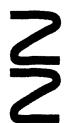
\includegraphics[keepaspectratio]{images/part001_fce77adb.jpg}}

Remarks. --- 1) A Cauchy sequence \((\mathbf{f}_n)\) in \(\mathcal{L}_{\mathrm{F}}^{p}\) can be such that the sequence \((\mathbf{f}_n(x))\) is not convergent at any point of X (Exer. 1).

\begin{enumerate}
\def\labelenumi{\arabic{enumi})}
\setcounter{enumi}{1}
\tightlist
\item
  If \(\mathbf{f}\) belongs to \(\mathcal{L}_{\mathrm{F}}^{p}\) , it is not always possible to find a sequence \((\mathbf{f}_n)\) of continuous functions with compact support such that the sequence \((\mathbf{f}_n(x))\) converges everywhere in \(X\) to a function equal to \(\mathbf{f}(x)\) almost everywhere (§4, Exer. 4 c)).
\end{enumerate}

\subsection{Properties of p-th power integrable functions}

THEOREM 4. --- Let F and G be two Banach spaces, u a continuous linear mapping of F into G. For every function \(f \in L_{F}^{p}\) , the composite function \(u \circ f\) belongs to \(L_{G}^{p}\) .

Let \(\mathbf{f} \in \mathcal{L}_{\mathrm{F}}^{p}\) ; for every \(\varepsilon > 0\) , there exists a function \(\mathbf{g} \in \mathcal{K}_{\mathrm{F}}\) such that \(\mathrm{N}_p(\mathbf{f} - \mathbf{g}) \leqslant \varepsilon\) ; since \(|\mathbf{u} \circ \mathbf{f} - \mathbf{u} \circ \mathbf{g}| \leqslant \| \mathbf{u} \| \cdot |\mathbf{f} - \mathbf{g}|\) , we have

\[
\mathrm{N} _ {p} (\mathbf {u} \circ \mathbf {f} - \mathbf {u} \circ \mathbf {g}) \leqslant \| \mathbf {u} \| \cdot \mathrm{N} _ {p} (\mathbf {f} - \mathbf {g}) \leqslant \varepsilon \| \mathbf {u} \|,
\]

and since \(u \circ g\) is continuous with compact support, the theorem is proved.

COROLLARY 1. --- Let \(\mathbf{a}'\) be a continuous linear form on \(\mathbf{F}\) ; if \(\mathbf{f} \in \mathcal{L}_{\mathrm{F}}^{p}\) , the numerical function \(x \mapsto \langle \mathbf{f}(x), \mathbf{a}' \rangle\) (denoted by \(\langle \mathbf{f}, \mathbf{a}' \rangle\) ) belongs to \(\mathcal{L}^p\) .

COROLLARY 2. --- Given \(n\) points \(\mathbf{a}_k\) of \(F (1 \leqslant k \leqslant n)\) , and \(n\) numerical functions \(f_k (1 \leqslant k \leqslant n)\) belonging to \(\mathcal{L}^p\) , the function \(\mathbf{f} = \sum_{k=1}^{n} \mathbf{a}_k f_k\) belongs to \(\mathcal{L}_F^p\) .

This follows from the fact that the mapping \(t \mapsto at\) of R into F is continuous.

PROPOSITION 9. --- Let F be an n-dimensional vector space over R, and let \((\mathbf{e}_{k})_{1\leqslant k\leqslant n}\) be a basis of F. For a function \(f=\sum_{k=1}^{n}\mathbf{e}_{k}f_{k}\) to belong to \(L_{F}^{p}\) , it is necessary and sufficient that each of the numerical functions \(f_{k}\) belong to \(L^{p}\) .

This follows at once from Cors. 1 and 2 of Th. 4.

PROPOSITION 10. --- In the space \(\mathcal{L}_{\mathrm{F}}^{p}\) , the linear subspace formed by the (finite) linear combinations \(\sum_{k} \mathbf{a}_{k} f_{k}\) , where \(\mathbf{a}_{k} \in \mathbf{F}\) and the \(f_{k}\) are continuous numerical functions with compact support, is dense (for the topology of convergence in mean of order \(p\) ).

The set \(H_{F}\) of continuous mappings of X into F with compact support is by definition dense in \(L_{F}^{p}\) . On the other hand, every function \(g \in H_{F}\) may be uniformly approximated by functions of the form \(\sum_{k} a_{k} f_{k}\) , where the \(f_{k}\) are continuous functions with support contained in a fixed compact neighborhood of the support of g (Ch. III, §1, No.~2, Lemma 2); it follows (No.~3, Prop. 4) that g is in the closure in \(L_{F}^{p}\) of the set of \(\sum_{k} a_{k} f_{k}\) , whence the proposition.

PROPOSITION 11. --- If a function f belongs to \(L_{F}^{p}\) , then the function \(|f|\) belongs to \(L^{p}\) , and the mapping \(f \mapsto |f|\) of \(L_{F}^{p}\) into \(L^{p}\) is uniformly continuous (for the topology of convergence in mean of order p).

For every \(\varepsilon > 0\) there exists a continuous function \(\mathbf{g}\) with compact support, such that \(\mathrm{N}_p(\mathbf{f} - \mathbf{g}) \leqslant \varepsilon\) ; since \(||\mathbf{f}| - |\mathbf{g}|| \leqslant |\mathbf{f} - \mathbf{g}|\) , we have \(\mathrm{N}_p(|\mathbf{f}| - |\mathbf{g}|) \leqslant \varepsilon\) , which proves that \(|\mathbf{f}| \in \mathcal{L}^p\) . On the other hand, if \(\mathbf{f}_1, \mathbf{f}_2\) are two functions in \(\mathcal{L}_{\mathrm{F}}^p\) then \(\mathrm{N}_p(|\mathbf{f}_1| - |\mathbf{f}_2|) \leqslant \mathrm{N}_p(\mathbf{f}_1 - \mathbf{f}_2)\) , which shows that \(\mathbf{f} \mapsto |\mathbf{f}|\) is a uniformly continuous mapping.

PROPOSITION 12. --- For a numerical function f to belong to \(L^{p}\) , it is necessary and sufficient that each of the functions \(f^{+}\) and \(f^{-}\) belong to \(L^{p}\) .

The condition is sufficient since \(f = f^{+} - f^{-}\) ; it is necessary, because if \(f \in \mathcal{L}^p\) then \(|f| \in \mathcal{L}^p\) (Prop. 11).

COROLLARY. --- The upper (resp. lower) envelope of a finite family of functions in \(\mathcal{L}^{p}\) belongs to \(\mathcal{L}^{p}\) .

\subsection{\texorpdfstring{Directed sets in \(L^{p}\) and increasing sequences in \(L^{p}\)}{Directed sets in L to the p and increasing sequences in L to the p}}

We have defined (§2, No.~6) an order relation \(\widetilde{f} \leqslant \widetilde{g}\) in the set \(\widetilde{\mathcal{F}}\) of equivalence classes of numerical functions defined and finite almost everywhere in \(X\) ; equipped with this order relation and with its vector space structure, \(\widetilde{\mathcal{F}}\) is a Riesz space. The corollary of Prop. 12 of No.~5 shows that if \(\widetilde{f}\) and \(\widetilde{g}\) are two elements of the subspace \(L to the p\) of \(\widetilde{\mathcal{F}}\) , then the supremum \(\sup (\widetilde{f}, \widetilde{g})\) of \(\widetilde{f}\) and \(\widetilde{g}\) in \(\widetilde{\mathcal{F}}\) (which is the class of each of the functions \(\sup (f, g)\) , where \(f \in \widetilde{f}\) and \(g \in \widetilde{g}\) ) belongs to \(L to the p\) ; this proves in particular that \(L to the p\) , equipped with the order relation induced by that of \(\widetilde{\mathcal{F}}\) , is a Riesz space.

PROPOSITION 13. --- In the Riesz space \(L^{p}\) , equipped with the topology defined by the norm \(\|f\|_{p}\) , the mapping \(\widetilde{f} \mapsto |f|\) is uniformly continuous, and the set of elements \(f \geqslant 0\) is closed.

The first part of the proposition follows at once from Prop. 11 of No.~5; since the set of \(\widetilde{f} \geqslant 0\) is also the set of \(\widetilde{f}\) such that \(|\widetilde{f}| = \widetilde{f}\) , it is closed, because \(\widetilde{f} \mapsto |\widetilde{f}|\) is a continuous mapping and \(\mathbf{L}^p\) is Hausdorff.

We thus see that the topology on \(L^{p}\) defined by the norm \(\|f\|_{p}\) is compatible with the ordered vector space structure of \(L^{p}\) (TVS, II, §2, No.~7).

PROPOSITION 14. --- Let H be a subset of the Riesz space \(L^{p}\) , consisting of classes \(\geqslant 0\) and directed for the relation \(\leqslant\) . For H to have a supremum in \(L^{p}\) , it is necessary and sufficient that

\[
\sup _ {\widetilde {f} \in \mathrm{H}} \| \widetilde {f} \| _ {p} <   + \infty .
\]

The supremum of H in \(L^{p}\) is then the limit (in the Banach space \(L^{p}\) ) of the section filter of H.

The condition is clearly necessary, since \(\widetilde{f} \mapsto \| \widetilde{f} \|_p\) is an increasing function on the set of elements \(\geqslant 0\) of \(L to the p\) . To see that it is sufficient, we first observe that it implies that the image of H under the mapping \(\widetilde{f} \mapsto \| \widetilde{f} \|_p\) has a limit in \(\mathbf{R}\) , by the monotone limit theorem; the image of the section filter \(\mathfrak{F}\) of H under this mapping is therefore a base of a Cauchy filter on \(\mathbf{R}\) . The proof will be complete if we show that \(\mathfrak{F}\) itself is a base of a Cauchy filter on \(L to the p\) ; for, \(\mathfrak{F}\) will then converge in \(L to the p\) , since \(L to the p\) is complete (No.~4, Th. 2), and the proposition will follow from TVS, II, §2, No.~7, Prop. 18.

To see that \(\mathfrak{F}\) is a base of a Cauchy filter, we shall make use of the following lemma:

Lemma. --- If \(f\) and \(g\) are two functions in \(\mathcal{L}^p\) such that \(0 \leqslant f \leqslant g\) , then

\[
\left(\mathrm{N} _ {p} (g - f)\right) ^ {p} \leqslant \left(\mathrm{N} _ {p} (g)\right) ^ {p} - \left(\mathrm{N} _ {p} (f)\right) ^ {p}.\tag{9}
\]

When \(f\) and \(g\) are continuous with compact support, the relation (9) may be written

\[
\int (g - f) ^ {p} d | \mu | \leqslant \int g ^ {p} d | \mu | - \int f ^ {p} d | \mu |
\]

and is then a consequence of the elementary inequality \((g - f)^{p} \leqslant g^{p} - f^{p}\) (No.~1, formula (2)). To pass from this to the general case, it suffices to observe that the two members of (9) are continuous functions on \(L^{p} \times L^{p}\) , and that every function \(f \geqslant 0\) in \(L^{p}\) is the limit (for convergence in mean of order p) of a sequence of continuous functions \(\geqslant 0\) with compact support, by the continuity of the mapping \(g \mapsto |g|\) on \(L^{p}\) (Prop. 11).

The lemma having been established, for every \(\varepsilon > 0\) there exists by hypothesis an \(\widetilde{f} \in \mathbf{H}\) such that, for every \(\widetilde{g} \geqslant \widetilde{f}\) belonging to \(\mathbf{H}\) , we have \((\|\widetilde{g}\|_p)^p - (\|\widetilde{f}\|_p)^p \leqslant \varepsilon\) ; from this it follows that \((\|\widetilde{g} - \widetilde{f}\|_p)^p \leqslant \varepsilon\) ; thus, if \(\widetilde{g}_1\) and \(\widetilde{g}_2\) are two elements in \(\mathbf{H}\) that are \(\geqslant \widetilde{f}\) , then \(\|\widetilde{g}_1 - \widetilde{g}_2\|_p \leqslant 2\varepsilon^{1/p}\) , which proves that \(\mathfrak{F}\) is a Cauchy filter base on \(\mathrm{L}^p\) and completes the proof of Prop. 14.

COROLLARY 1. --- If \(\widetilde{g}\) is the supremum of H in \(\mathbf{L}^p\) , then

\[
\| \widetilde {g} \| _ {p} = \lim _ {\widetilde {f} \in \mathrm{H}} \| \widetilde {f} \| _ {p} = \sup _ {\widetilde {f} \in \mathrm{H}} \| \widetilde {f} \| _ {p}.\tag{10}
\]

This follows from the continuity of the norm \(\|\widetilde{f}\|_{p}\) in \(L^{p}\) , and the monotone limit theorem.

COROLLARY 2. --- The Riesz space \(L^{p}\) is fully lattice-ordered.

Every directed set H in \(L^{p}\) (for the relation \(\leqslant\) ), consisting of classes \(\geqslant 0\) and bounded above in \(L^{p}\) , has a supremum: for, if \(\widetilde{h}\) is an upper bound for H in \(L^{p}\) , then \(\|f\|_{p} \leqslant \|h\|_{p}\) for all \(\widetilde{f} \in H\) , and Prop. 14 is applicable. This proves the corollary (Ch. II, §1, No.~3, Prop. 1).

The conclusions of Prop. 14 no longer hold when they are formulated for the functions in \(\mathcal{L}^p\) instead of their classes. To be precise, if M is a subset of \(\mathcal{L}^p\) , consisting of functions \(\geqslant 0\) , directed for the relation \(\leqslant\) , and such that \(\sup_{f\in\mathbb{M}}\mathrm{N}_{p}(f)<+\infty\) , the class of the upper envelope \(g\) of M is not

necessarily identical to the supremum in \(\mathrm{L}^p\) of the classes of the functions \(f \in \mathbf{M}\) ; in particular, \(g\) is not necessarily \(p\) -th power integrable, and even if \(g \in \mathcal{L}^p\) , \(\mathrm{N}_p(g)\) can be distinct from \(\sup_{f \in \mathbf{M}} \mathrm{N}_p(f)\) (cf.~§1, No.~3, Remark 1 following Th. 3).

Nevertheless, we have the following theorem:

THEOREM 5. --- Let \((f_n)\) be an increasing sequence of functions \(\geqslant 0\) in \(\mathcal{L}^p\) . For the upper envelope \(f\) of this sequence to be \(p\) -th power integrable, it is necessary and sufficient that \(\sup_{n} N sub p(f_n) < +\infty\) . The sequence \((f_n)\) is then convergent in mean of order \(p\) to \(f\) , and

\[
\mathrm{N} _ {p} (f) = \sup _ {n} \mathrm{N} _ {p} (f _ {n}) = \lim _ {n \rightarrow \infty} \mathrm{N} _ {p} (f _ {n}).\tag{11}
\]

The condition being obviously necessary, we need only prove that it is sufficient. Now, if the condition is satisfied then Prop. 14 shows that the sequence \((\tilde{f}_n)\) is a Cauchy sequence in \(L to the p\) , therefore the sequence \((f_n)\) is a Cauchy sequence in \(\mathcal{L}^p\) ; since \(f_n(x)\) tends to \(f(x)\) for all \(x \in X\) , \(f\) is \(p\) -th power integrable and is the limit of the sequence \((f_n)\) for the topology of convergence in mean of order \(p\) (No.~4, Cor. 1 of Th. 3). Therefore \(\mathrm{N}_p(f_n)\) tends to \(\mathrm{N}_p(f)\) since \(\mathrm{N}_p\) is a continuous function on \(\mathcal{L}^p\) .

COROLLARY 1. --- Let \((f_n)\) be a decreasing sequence of functions \(\geqslant 0\) in \(\mathcal{L}^p\) ; then, the lower envelope \(f\) of the sequence belongs to \(\mathcal{L}^p\) , the sequence \((f_n)\) converges in mean of order \(p\) to \(f\) , and

\[
\mathrm{N} _ {p} (f) = \lim _ {n \rightarrow \infty} \mathrm{N} _ {p} (f _ {n}) = \inf _ {n} \mathrm{N} _ {p} (f _ {n}).
\]

The first two assertions follow from Th. 5 applied to the sequence \(g_{n} = f_{1} - f_{n}\) , which is increasing and bounded above; the rest is then obvious.

COROLLARY 2. --- Let \((f_n)\) be a sequence of functions in \(\mathcal{L}^p\) . For the upper envelope \(f\) of the sequence \((f_n)\) to be \(p\) -th power integrable, it is necessary and sufficient that there exist a function \(g \geqslant 0\) such that \(\int^{*} g^p d|\mu| < +\infty\) and \(f_n \leqslant g\) for all \(n\) .

The condition is obviously necessary, on taking \(g = f^{+}\) . Conversely, suppose it is verified, and set \(g_{n} = \sup_{k\leqslant n}f_{k}\) ; the sequence \((g_{n})\) is increasing and consists of \(p\) -th power integrable functions (No.~5, Cor. of Prop. 12). The increasing sequence of positive functions \(h_n = g_n + g_1^-\) satisfies the conditions of Th. 5, since \(\mathrm{N}_p(h_n)\leqslant \mathrm{N}_p(g + g_1^-) < +\infty\) ; its upper envelope \(\sup_{n}h_{n}\) is therefore \(p\) -th power integrable, and the same is true of \(f = \sup_{n}h_{n} - g_{1}^{-}\) .

COROLLARY 3. --- Let A be a countable set, \(\mathfrak{F}\) a filter on A having a countable base, \((f_{\alpha})_{\alpha \in \mathrm{A}}\) a family of functions \(\geqslant 0\) in \(\mathcal{L}^p\) . Assume that there exists a function \(g \geqslant 0\) such that \(\mathrm{N}_p(g) < +\infty\) and \(f_{\alpha} \leqslant g\) for all \(\alpha \in \mathrm{A}\) ; then the function \(\limsup_{\mathfrak{F}} f_{\alpha}\) is \(p\) -th power integrable and

\[
\limsup _ {\mathfrak {F}} \mathrm{N} _ {p} (f _ {\alpha}) \leqslant \mathrm{N} _ {p} (\limsup _ {\mathfrak {F}} f _ {\alpha}).\tag{12}
\]

Let \((\mathbf{A}_n)\) be a decreasing base of \(\mathfrak{F}\) and set \(g_{n} = \sup_{\alpha \in \mathbf{A}_{n}}f_{\alpha}\) ; since \(\mathbf{A}_n\) is a countable set, it follows from Cor. 2 that \(g_{n}\) is \(p\) -th power integrable; on the other hand, \(\mathrm{N}_p(g_n)\geqslant \sup_{\alpha \in \mathbf{A}_n}\mathrm{N}_p(f_\alpha)\) . This being so, \(\limsup_{\mathfrak{F}}f_{\alpha}\) is the lower envelope of the decreasing sequence \((g_n)\) ; thus \(\limsup_{\mathfrak{F}}f_{\alpha}\) is \(p\) -th power integrable by Cor. 1, and

\[
\begin{array}{l} \mathrm{N} _ {p} (\limsup _ {\mathfrak {F}} f _ {\alpha}) = \mathrm{N} _ {p} \left(\inf _ {n} g _ {n}\right) = \lim _ {n \to \infty} \mathrm{N} _ {p} (g _ {n}) \\ \geqslant \lim _ {n \to \infty} \left(\sup _ {\alpha \in \mathrm{A} _ {n}} \mathrm{N} _ {p} (f _ {\alpha})\right) = \limsup _ {\mathfrak {F}} \mathrm{N} _ {p} (f _ {\alpha}). \end{array}
\]

\subsection{Lebesgue's theorem}

THEOREM 6 (Lebesgue). --- Let F be a Banach space, \((\mathbf{f}_{n})\) a sequence of functions in \(L_{F}^{p}\) such that: \(1^{\circ}\) the sequence \((\mathbf{f}_{n}(x))\) converges almost everywhere to a limit \(\mathbf{f}(x) \in \mathrm{F}\) ; \(2^{\circ}\) there exists a numerical function \(g \geqslant 0\) such that \(\int^{*} g^{p} d|\mu| < +\infty\) and \(|\mathbf{f}_{n}(x)| \leqslant g(x)\) almost everywhere in X, for every integer n.~Then, the function f (defined almost everywhere) is p-th power integrable, and the sequence \((\mathbf{f}_{n})\) converges in mean of order p to f.

Consider the `double' sequence of numerical functions \(g_{mn} = |\mathbf{f}_m - \mathbf{f}_n|\) , which belong to \(\mathcal{L}^p\) (No.~5, Prop. 11); by hypothesis, \(\lim_{m\to \infty, n\to \infty}g_{mn}(x) = 0\) almost everywhere, and on the other hand \(|g_{mn}(x)|\leqslant 2g(x)\) almost everywhere; applying Cor. 3 of Th. 5 of No.~6 to this double sequence,

\[
\limsup _ {m \to \infty ,   n \to \infty} \mathrm{N} _ {p} (\mathbf {f} _ {m} - \mathbf {f} _ {n}) \leqslant \mathrm{N} _ {p} (0) = 0  ,
\]

and since \(\mathrm{N}_p(\mathbf{f}_m - \mathbf{f}_n) \geqslant 0\) this implies \(\lim_{m \to \infty, n \to \infty} \mathrm{N}_p(\mathbf{f}_m - \mathbf{f}_n) = 0\) ; in other words, the sequence \((\mathbf{f}_n)\) is a Cauchy sequence in \(\mathcal{L}_{\mathrm{F}}^p\) . The theorem therefore follows from Cor. 1 of Th. 3 of No.~4.

COROLLARY. --- Let A be a set of indices, filtered by a filter F having a countable base. If \((\mathbf{f}_{\alpha})_{\alpha \in \mathrm{A}}\) is a family of functions in \(L_{F}^{p}\) that, with respect to the filter \(\mathfrak{F}\) , converge pointwise almost everywhere to a function \(\mathbf{f}\) , and if, moreover, there exists a numerical function \(g \geqslant 0\) such that \(\int^{*} g^{p} d|\mu| < +\infty\) and \(|\mathbf{f}_{\alpha}(x)| \leqslant g(x)\) almost everywhere in \(X\) for each \(\alpha \in A\) , then the function \(\mathbf{f}\) is \(p\) -th power integrable and \(\mathbf{f}_{\alpha}\) tends in mean of order \(p\) to \(\mathbf{f}\) with respect to the filter \(\mathfrak{F}\) .

For, let \((\mathbf{A}_{n})\) be a decreasing countable base of F, and let \(\alpha_{n}\) be any element of \(A_{n}\) ; the sequence \((\mathbf{f}_{\alpha_{n}})\) converges pointwise to f almost everywhere in X, thus Th. 6 shows that f is p-th power integrable and that \(\lim_{n\to\infty}\mathrm{N}_{p}(\mathbf{f}-\mathbf{f}_{\alpha_{n}})=0\) . Since F is the intersection filter of the elementary filters associated with all such sequences \((\alpha_{n})\) (GT, I, §6, No.~8, Prop. 11), \(\lim_{\mathfrak{F}}\mathrm{N}_{p}(\mathbf{f}-\mathbf{f}_{\alpha})\) exists and is equal to the common limit 0 of all of the sequences \((\mathrm{N}_{p}(\mathbf{f}-\mathbf{f}_{\alpha_{n}}))\) .

\pandocbounded{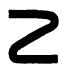
\includegraphics[keepaspectratio]{images/part001_1313f7e2.jpg}}

Remarks. --- 1) Th. 6 no longer holds if the hypothesis \(|\mathbf{f}_n| \leqslant g\) (with \(\mathrm{N}_p(g) < +\infty\) ) is replaced by the weaker hypothesis \(\sup_{n} \mathrm{N}_p(\mathbf{f}_n) < +\infty\) . Suppose, for example, that \(\mu\) is Lebesgue measure on \(\mathbf{R}\) ; define continuous functions \(f_n\) in the following manner: \(f_n(x) = 0\) for \(x \leqslant 0\) and for \(x \geqslant \frac{2}{n}\) , \(f_n(\frac{1}{n}) = n\) , \(f_n\) being linear on the intervals \([0, \frac{1}{n}]\) and \([\frac{1}{n}, \frac{2}{n}]\) . Then \(\lim_{n \to \infty} f_n(x) = 0\) for all \(x \in \mathbf{R}\) , but \(\mathrm{N}_1(f_n) = 1\) for every \(n\) (cf.~§5, Exer. 12).

\pandocbounded{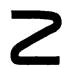
\includegraphics[keepaspectratio]{images/part001_8f7b1086.jpg}}

\begin{enumerate}
\def\labelenumi{\arabic{enumi})}
\setcounter{enumi}{1}
\tightlist
\item
  The Cor. of Th. 6 no longer holds if it is not assumed that the filter \(\mathfrak{F}\) has a countable base (cf.~§1, No.~3, Remark 1 following the Cor. of Th. 3).
\end{enumerate}

\subsection{\texorpdfstring{Relations between the spaces \(L_{F}^{p}\) ( \(1 \leqslant p < +\infty\) )}{Relations between the spaces L sub F to the p ( 1 <= p < +infinity )}}

For every real number \(\alpha > 0\) , the mapping \(z \mapsto |z|^{\alpha-1} \cdot z\) is defined and continuous on the complement of 0 in F; moreover, since \(\left||z|^{\alpha-1} \cdot z\right| = |z|^{\alpha}\) , this function tends to 0 with z and may therefore be extended by continuity to the point 0 by giving it the value 0 at this point, even if \(\alpha < 1\) .

THEOREM 7. --- Let p and q be two real numbers such that \(1 \leqslant p < +\infty\) , \(1 \leqslant q < +\infty\) . If a function f belongs to \(L_{F}^{p}\) then the function \(|f|^{(p/q)-1} \cdot f\) belongs to \(L_{F}^{q}\) , and conversely.

By hypothesis, there exists a sequence \((\mathbf{f}_{n})\) of continuous functions with compact support such that \(\sum_{n=1}^{\infty}\mathrm{N}_{p}(\mathbf{f}_{n})<+\infty\) and \(\mathbf{f}(x)=\sum_{n=1}^{\infty}\mathbf{f}_{n}(x)\) almost everywhere (No.~4, Th. 3). Set

\[
\mathbf {g} _ {n} = | \mathbf {f} _ {1} + \mathbf {f} _ {2} + \dots + \mathbf {f} _ {n} | ^ {(p / q) - 1} \cdot (\mathbf {f} _ {1} + \mathbf {f} _ {2} + \dots + \mathbf {f} _ {n});
\]

the function \(g_{n}\) is continuous with compact support; on the other hand,

\[
\left| \mathbf {g} _ {n} \right| ^ {q} = \left| \mathbf {f} _ {1} + \mathbf {f} _ {2} + \dots + \mathbf {f} _ {n} \right| ^ {p} \leqslant \left(\sum_ {n = 1} ^ {\infty} \left| \mathbf {f} _ {n} \right|\right) ^ {p} = h ^ {q},
\]

where the numerical function \(h \geqslant 0\) (finite or not) satisfies the inequality

\[
\left(\mathrm{N} _ {q} (h)\right) ^ {q} = \left(\mathrm{N} _ {p} \left(\sum_ {n = 1} ^ {\infty} | \mathbf {f} _ {n} |\right)\right) ^ {p} \leqslant \left(\sum_ {n = 1} ^ {\infty} \mathrm{N} _ {p} (\mathbf {f} _ {n})\right) ^ {p} <   + \infty
\]

by the countable convexity theorem. Moreover, \(\mathbf{g}_n(x)\) tends almost everywhere to \(\mathbf{g}(x) = |\mathbf{f}(x)|^{(p/q)-1} \cdot \mathbf{f}(x)\) , therefore Lebesgue's theorem shows that \(\mathbf{g} \in \mathcal{L}_{\mathrm{F}}^q\) . The converse is immediate, since \(\mathbf{f} = |\mathbf{g}|^{(q/p)-1} \cdot \mathbf{g}\) .

It can be shown that the mapping \(\mathbf{f} \mapsto |\mathbf{f}|^{\frac{p}{q}-1} \cdot \mathbf{f}\) is a homeomorphism of \(\mathcal{L}_{\mathrm{F}}^{p}\) onto \(\mathcal{L}_{\mathrm{F}}^{q}\) (§6, Exer. 10).

COROLLARY 1. --- For a function \(\mathbf{f}\) to belong to \(\mathcal{L}_{\mathrm{F}}^{p}\) , it is necessary and sufficient that the function \(|\mathbf{f}|^{p-1} \cdot \mathbf{f}\) belong to \(\mathcal{L}_{\mathrm{F}}^{1}\) .

COROLLARY 2. --- For a positive numerical function f to belong to \(L^{p}\) , it is necessary and sufficient that \(f^{p}\) belong to \(L^{1}\) .

\pandocbounded{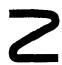
\includegraphics[keepaspectratio]{images/part001_881031c4.jpg}}

Note that if \(f\) is a numerical function of arbitrary sign, such that \(|f|^p\) belongs to \(\mathcal{L}^1\) , \(f\) does not necessarily belong to \(\mathcal{L}^p\) (cf.~§4, Exer. 8).

\section{INTEGRABLE FUNCTIONS AND SETS}

\subsection{Extension of the integral}

It follows from the definition of the space \(L_{F}^{p}\) that the subspace \(H_{F}\) of continuous functions with compact support is dense in \(L_{F}^{p}\) (§3, No.~4, Def. 2). Every continuous (for the topology of convergence in mean of order p) linear function, defined on \(H_{F}\) and taking its values in a complete Hausdorff topological vector space G, can therefore be extended by continuity in a unique manner, to a continuous linear function defined on \(L_{F}^{p}\) with values in G (GT, II, §3, No.~6, Th. 2 and III, §3, No.~1, Prop. 3).

Now, for every continuous function \(\mathbf{f}\) with compact support, with values in the Banach space \(\mathrm{F}\) , we have defined (in Ch. III, §3, No.~1) the integral \(\mu(\mathbf{f}) = \int \mathbf{f} d\mu\) with respect to \(\mu\) , which is an element of \(\mathrm{F}\) , and we have proved (Ch. III, §3, No.~2, Prop. 6) the inequality

\[
\left| \int \mathbf {f} d \mu \right| \leqslant \int | \mathbf {f} | d | \mu | = \mathrm{N} _ {1} (\mathbf {f}).\tag{1}
\]

This inequality proves that the linear mapping \(\mathbf{f} \mapsto \int \mathbf{f} d\mu\) of \(\mathcal{H}_{\mathrm{F}}\) into \(\mathrm{F}\) is continuous for the topology of convergence in mean in \(\mathcal{H}_{\mathrm{F}}\) . It can therefore be extended by continuity to the entire space \(L_{F}^{1}\) , and we may make the following definition:

DEFINITION 1. --- The functions belonging to \(\mathcal{L}_{\mathrm{F}}^{1}(\mathrm{X},\mu)\) are said to be integrable with respect to the measure \(\mu\) (or, again, that they are \(\mu\) -integrable). The integral (with respect to \(\mu\) ) of the integrable function \(\mathbf{f}\) is by definition the value at \(\mathbf{f}\) of the extension by continuity to \(\mathcal{L}_{\mathrm{F}}^{1}\) of the linear mapping \(\mathbf{g} \mapsto \int \mathbf{g} d\mu\) of \(\mathcal{K}_{\mathrm{F}}\) into \(\mathrm{F}\) ; it is again denoted \(\mu(\mathbf{f})\) or \(\int \mathbf{f} d\mu\) , or \(\int \mathbf{f}(x) d\mu(x)\) or \(\int \mathbf{f}\mu\) , or \(\int \mathbf{f}(x)\mu(x)\) .

Example. --- Let X be a discrete space, \(\mu\) a measure on X, and set \(\alpha(x) = \mu(\varphi_{\{x\}})\) for every \(x \in X\) . The functions in \(F_{F}^{1}\) are then integrable, in other words \(L_{F}^{1} = F_{F}^{1}\) ; moreover, for every function \(f \in L_{F}^{1}\) ,

\[
\int \mathbf {f} d \mu = \sum_ {x \in X} \alpha (x) \mathbf {f} (x).
\]

For, let \(\mathbf{f} \in \mathcal{F}_F^1\) ; we have \(|\mu|^*(|\mathbf{f}|) = \sum_{x \in X} |\alpha(x)| \cdot |\mathbf{f}(x)| < +\infty\) (§1, No.~3, Example); for every \(\varepsilon > 0\) , there exists a finite subset \(M\) of \(X\) such that

\[
\sum_ {x \in \mathrm{X} - \mathrm{M}} | \alpha (x) | \cdot | \mathbf {f} (x) | \leqslant \varepsilon .
\]

The function \(\mathbf{g}\) equal to \(\mathbf{f}\) at the points \(x\in M\) where \(|\mathbf{f}|\) is finite, and to 0 elsewhere, belongs to \(\mathcal{H}(\mathrm{X};\mathrm{F})\) and, by the conventions that have been made,

\[
| \mu | ^ {*} (| \mathbf {f} - \mathbf {g} |) \leqslant \sum_ {\boldsymbol {x} \in \mathrm{X} - \mathrm{M}} | \alpha (\boldsymbol {x}) | \cdot | \mathbf {f} (\boldsymbol {x}) | \leqslant \varepsilon ,
\]

which proves that \(\mathbf{f} \in \mathcal{L}_{\mathrm{F}}^{1}\) . On the other hand,

\[
\left| \mu (\mathbf {g}) - \sum_ {x \in X} \alpha (x) \mathbf {f} (x) \right| \leqslant \sum_ {x \in X - M} | \alpha (x) | \cdot | \mathbf {f} (x) | \leqslant \varepsilon ,
\]

whence the second assertion.

In other words, the \(\mu\) -integrable functions \(\mathbf{f}\) are those for which the family \((\alpha(x)\mathbf{f}(x))_{x\in X}\) is absolutely summable (GT, IX, §3, No.~6), and the integral \(\int \mathbf{f} d\mu\) is the sum of this family.

Since \(\mu(\mathbf{f})\) is continuous on \(\mathcal{L}_{\mathrm{F}}^{1}\) by definition, and since it takes its values in a Hausdorff space, we have \(\mu(\mathbf{f}) = 0\) for every function that belongs to the closure of 0 in \(\mathcal{L}_{\mathrm{F}}^{1}\) , that is, is negligible; if \(\mathbf{f}\) and \(\mathbf{g}\) are two equivalent integrable functions, then \(\mu(\mathbf{f}) = \mu(\mathbf{g})\) . In other words, the value of \(\mu(\mathbf{f})\) depends only on the class \(\widetilde{\mathbf{f}}\) of the integrable function \(\mathbf{f}\) ; it is again denoted \(\mu(\widetilde{\mathbf{f}})\) , and the function \(\widetilde{\mathbf{f}} \mapsto \mu(\widetilde{\mathbf{f}})\) is a continuous linear mapping of \(L_{F}^{1}\) into F. If a function f, with values in F and defined almost everywhere in X, is equivalent to an integrable function, we again say that f is integrable and we write \(\int f d\mu = \mu(\widetilde{\mathbf{f}})\) ; one defines similarly an integrable function with values in \(\overline{R}\) , defined and finite almost everywhere, as well as its integral.

\subsection{Properties of the integral}

PROPOSITION 1. --- For every positive \(\mu\) -integrable numerical function \(f\) ,

\[
\int f d | \mu | = \int^ {*} f d | \mu | = \mathrm{N} _ {1} (f) \geqslant 0.\tag{2}
\]

For, \(\int f d|\mu|\) and \(\mathrm{N}_{1}(f)\) are continuous on \(L^{1}\) and are equal for every continuous function \(f \geqslant 0\) with compact support; on the other hand, every function \(f \geqslant 0\) in \(L^{1}\) is the limit (in the sense of convergence in mean) of a sequence of continuous functions \(\geqslant 0\) with compact support ( \(\S3\) , No.~5, Prop. 11); whence the proposition.

COROLLARY 1. --- For every integrable function \(\mathbf{f} \in \mathcal{L}_{\mathrm{F}}^{1}\) , \(|\mathbf{f}|\) is integrable and

\[
\int | \mathbf {f} | d | \mu | = \int^ {*} | \mathbf {f} | d | \mu | = \mathrm{N} _ {1} (\mathbf {f}).\tag{3}
\]

We shall make frequent use of Prop. 1 and its Cor. 1, on replacing \(\int^{*}fd|\mu|\) or \(\mathrm{N}_{1}(f)\) by \(\int fd|\mu|\) when dealing with an integrable function \(\geqslant 0\) . For example, for two integrable functions \(\mathbf{f},\mathbf{g}\) to be equivalent, it is necessary and sufficient that \(\int |\mathbf{f} - \mathbf{g}|d|\mu| = 0\) .

We recall that, for a function \(\mathbf{f}\) to belong to \(\mathcal{L}_{\mathrm{F}}^{p}\) , it is necessary and sufficient that the function \(|\mathbf{f}|^{p - 1}\cdot \mathbf{f}\) belong to \(\mathcal{L}_{\mathrm{F}}^{1}\) (§3, No.~8, Cor. 1 of Th. 7), that is, that it be integrable; this is the reason for the terminology ' \(p\) -th power integrable function'. Moreover:

COROLLARY 2. --- For every function \(\mathbf{f} \in \mathcal{L}_{\mathrm{F}}^{p}\) , the numerical function \(|\mathbf{f}|^{p}\) is integrable and

\[
\mathrm{N} _ {p} (\mathbf {f}) = \left(\int | \mathbf {f} | ^ {p} d | \mu |\right) ^ {1 / p}.\tag{4}
\]

This follows at once from the fact that \(|\mathbf{f}|\) belongs to \(\mathcal{L}^p\) (§3, No.~5, Prop. 11) and formula (2).

PROPOSITION 2. --- For every integrable function f,

\[
\left| \int \mathbf {f} d \mu \right| \leqslant \int | \mathbf {f} | d | \mu |.\tag{5}
\]

This follows at once from the inequality (1) by passage to the limit, on taking into account (3) and the continuity of \(\mathrm{N}_{1}(\mathbf{f})\) on \(L_{F}^{1}\) .

THEOREM 1. --- Let F and G be two Banach spaces, u a continuous linear mapping of F into G. For every integrable function f with values in F, \(u \circ f\) is integrable and

\[
\int \mathbf {u} (\mathbf {f} (x)) d \mu (x) = \mathbf {u} \left(\int \mathbf {f} (x) d \mu (x)\right).\tag{6}
\]

We already know that \(\mathbf{u} \circ \mathbf{f}\) is integrable (§3, No.~5, Th. 4); the relation (6), being valid for every \(\mathbf{f} \in \mathcal{K}_{\mathrm{F}}\) , extends to every integrable function \(\mathbf{f}\) by the principle of extension of identities: for, \(\mathbf{f} \mapsto \mathbf{u} \circ \mathbf{f}\) is continuous for the topology of convergence in mean, as follows from the inequality \(\mathrm{N}_1(\mathbf{u} \circ \mathbf{f}) \leqslant \| \mathbf{u} \| \cdot \mathrm{N}_1(\mathbf{f})\) .

COROLLARY 1. --- Let \(\mathbf{a}'\) be a continuous linear form on \(\mathbf{F}\) . If \(\mathbf{f}\) is an integrable function with values in \(\mathbf{F}\) , then the numerical function \(\langle \mathbf{f}, \mathbf{a}' \rangle\) is integrable and

\[
\int \left\langle \mathbf {f} (x), \mathbf {a} ^ {\prime} \right\rangle d \mu (x) = \left\langle \int \mathbf {f} (x) d \mu (x), \mathbf {a} ^ {\prime} \right\rangle .\tag{7}
\]

We shall see in Ch. VI, §1, Exers. 7, 11 and 12 that there can exist functions \(\mathbf{f}\) , with values in an infinite-dimensional Banach space \(\mathbf{F}\) , such that \(\langle \mathbf{f}, \mathbf{a}' \rangle\) is integrable for every continuous linear form \(\mathbf{a}'\) on \(\mathbf{F}\) , without \(\mathbf{f}\) being integrable.

COROLLARY 2. --- If the \(\mathbf{a}_k\) ( \(1 \leqslant k \leqslant n\) ) are vectors in F and the \(f_k\) ( \(1 \leqslant k \leqslant n\) ) are integrable numerical functions, then the function \(\mathbf{f} = \sum_{k=1}^{n} \mathbf{a}_k f_k\) is integrable and

\[
\int \left(\sum_ {k = 1} ^ {n} \mathbf {a} _ {k} f _ {k}\right) d \mu = \sum_ {k = 1} ^ {n} \mathbf {a} _ {k} \int f _ {k} d \mu .\tag{8}
\]

\subsection{Passage to the limit in integrals}

PROPOSITION 3. --- Let B be a filter base on \(L_{F}^{1}\) . Assume that there exists a compact set \(K \subset X\) such that, for every set \(M \in B\) , all of the functions \(f \in M\) have their support in K. Under these conditions, if B converges uniformly on X to \(f_{0}\) , then the function \(f_{0}\) is integrable and

\[
\int \mathbf {f} _ {0} d \mu = \lim _ {\mathfrak {B}} \int \mathbf {f} d \mu .\tag{9}
\]

For, \(\mathfrak{B}\) converges in mean to \(\mathbf{f}_0\) (§3, No.~3, Prop. 4).

PROPOSITION 4. --- Let \((f_n)\) be an increasing (resp. decreasing) sequence of integrable numerical functions. For the upper (resp. lower) envelope \(f\) of the sequence to be integrable, it is necessary and sufficient that \(\sup_{n} \int f_n d|\mu| < +\infty\) (resp. \(\inf_{n} \int f_n d|\mu| > -\infty\) ), in which case

\[
\int f d \mu = \lim _ {n \to \infty} \int f _ {n} d \mu .\tag{10}
\]

We limit ourselves to considering an increasing sequence. The sequence \(g_{n} = f_{n} + f_{1}^{-}\) is increasing and consists of integrable functions \(\geqslant 0\) ; since its upper envelope is \(g = f + f_{1}^{-}\) , the proposition follows from Th. 5 of §3, No.~6.

THEOREM 2. --- Let A be a set of indices, filtered by a filter F with a countable base. Let \((\mathbf{f}_{\alpha})_{\alpha\in\mathrm{A}}\) be a family of integrable functions that, with respect to the filter F, converge pointwise almost everywhere to a function f; if there exists a numerical function \(g\geqslant0\) such that \(\int^{*}gd|\mu|<+\infty\) and such that \(|\mathbf{f}_{\alpha}(x)|\leqslant g(x)\) almost everywhere in X for each \(\alpha\in A\) , then the function f is integrable and

\[
\int \mathbf {f} d \mu = \lim _ {\mathfrak {F}} \int \mathbf {f} _ {\alpha} d \mu .\tag{11}
\]

The theorem follows from Lebesgue's theorem (§3, No.~7, Cor. of Th. 6) since, under the conditions of the statement, \(\mathbf{f}_{\alpha}\) converges in mean to \(\mathbf{f}\) with respect to \(\mathfrak{F}\) .

COROLLARY 1. --- Let \(\Omega\) be a topological space, \(t_0\) a point of \(\Omega\) admitting a countable fundamental system of neighborhoods, \(\mathbf{f}\) a mapping of \(\mathbf{X} \times \Omega\) into \(\mathbf{F}\) having the following properties:

\begin{enumerate}
\def\labelenumi{\alph{enumi})}
\item
  for every \(t \in \Omega\) , the function \(x \mapsto \mathbf{f}(x, t)\) is integrable;
\item
  for every \(x \in \mathrm{X}\) , the function \(t \mapsto \mathbf{f}(x, t)\) is continuous at \(t_0\) ;
\item
  there exist a neighborhood U of \(t_0\) and a numerical function \(g \geqslant 0\) defined on X, such that \(\int^{*} g d|\mu| < +\infty\) and \(|\mathbf{f}(x,t)| \leqslant g(x)\) for all \(x \in X\) and \(t \in U\) .
\end{enumerate}

Under these conditions, the mapping \(t \mapsto \int \mathbf{f}(x,t) d\mu(x)\) of \(\Omega\) into \(\mathbf{F}\) is continuous at the point \(t_0\) .

COROLLARY 2. --- Let \((\mathbf{f}_{n})\) be a sequence of integrable functions such that the series with general term \(\mathbf{f}_{n}(x)\) converges almost everywhere; if there exists a function \(g \geqslant 0\) such that \(\int^{*} g d|\mu| < +\infty\) and such that, for every integer n, \(\left|\sum_{k=1}^{n} \mathbf{f}_{k}(x)\right| \leqslant g(x)\) almost everywhere, then the sum \(\mathbf{f}(x)\) (defined almost everywhere) of the series with general term \(\mathbf{f}_{n}(x)\) is integrable and

\[
\int \mathbf {f} d \mu = \sum_ {n = 1} ^ {\infty} \int \mathbf {f} _ {n} d \mu\tag{12}
\]

(`term-by-term integration of a series').

\subsection{Characterizations of integrable numerical functions}

PROPOSITION 5. --- For a numerical function \(f \geqslant 0\) (finite or not), lower semi-continuous on X, to be integrable, it is necessary and sufficient that \(\int^{*} f d|\mu| < +\infty\) .

It all comes down to proving that the condition is sufficient. The definition of \(|\mu|^*(f)\) (§1, No.~1, Def. 1) proves that, for every \(\varepsilon > 0\) , there exists a continuous function \(g \geqslant 0\) , with compact support, such that \(g \leqslant f\) and \(|\mu|^*(f) \leqslant |\mu|(g) + \varepsilon\) . But \(f - g\) is lower semi-continuous and \(\geqslant 0\) , therefore (§1, No.~1, Th. 2)

\[
| \mu | ^ {*} (f) = | \mu | (g) + | \mu | ^ {*} (f - g),
\]

in other words \(\mathrm{N}_{1}(f-g)=|\mu|^{*}(f-g)=|\mu|^{*}(f)-|\mu|(g)\leqslant\varepsilon\) , which proves that f is integrable (§3, No.~4, Prop. 7).

COROLLARY 1. --- For a finite numerical function \(f \geqslant 0\) , upper semi-continuous on X, to be integrable, it is necessary and sufficient that \(\int^{*} f d|\mu| < +\infty\) .

For, if \(|\mu|^*(f) < +\infty\) , then there exists a lower semi-continuous function \(h\) such that \(f \leqslant h\) and \(|\mu|^*(h) < +\infty\) ; \(h - f\) is everywhere defined and lower semi-continuous, and \(|\mu|^*(h - f) \leqslant |\mu|^*(h) < +\infty\) ; therefore \(h - f\) is integrable, and since \(f(x) = h(x) - (h(x) - f(x))\) almost everywhere, \(f\) is integrable.

COROLLARY 2. --- Let H be a nonempty set, directed for the relation \(\leqslant (\text{resp. } \geqslant)\) , of lower (resp. upper) semi-continuous and integrable numerical functions; if

\[
\sup _ {f \in \mathrm{H}} \int f d | \mu | <   + \infty \quad (\mathrm{resp.} \inf _ {f \in \mathrm{H}} \int f d | \mu | > - \infty),
\]

then the upper (resp. lower) envelope g of H is integrable,

\[
\int g d \mu = \lim _ {f \in \mathrm{H}} \int f d \mu ,
\]

and \(\int g d|\mu| = \sup_{f\in \mathrm{H}}\int f d|\mu|\) (resp. \(\int g d|\mu| = \inf_{f\in \mathrm{H}}\int f d|\mu|\) ).

We may limit ourselves to the case of lower semi-continuous functions; the functions \(f^{+}\) (resp. \(f^{-}\) ), as \(f\) runs over \(\mathbf{H}\) , then form a directed set for \(\leqslant (\text{resp. } \geqslant)\) of lower (resp. upper) semi-continuous functions \(\geqslant 0\) ; the upper (resp. lower) envelope of the \(f^{+}\) (resp. \(f^{-}\) ), for \(f \in \mathbf{H}\) , is equal to \(g^{+}\) (resp. \(g^{-}\) ). On the other hand, one can replace \(\mathbf{H}\) by one of its sections (which is cofinal to it), consisting of the \(f \in \mathbf{H}\) that are \(\geqslant f_{0}\) , for some function \(f_{0} \in \mathbf{H}\) ; then \(\int f^{+} d|\mu| \leqslant \int f d|\mu| + \int f_{0}^{-} d|\mu|\) ; we thus see that we are reduced to proving the two assertions of the corollary when \(\mathbf{H}\) consists of positive functions. If \(\mathbf{H}\) is directed for \(\leqslant\) and consists of lower semi-continuous functions \(\geqslant 0\) , then we know (§1, No.~1, Th. 1) that

\[
| \mu | ^ {*} (g) = \sup _ {f \in \mathrm{H}} | \mu | ^ {*} (f) = \sup _ {f \in \mathrm{H}} \int f d | \mu | <   + \infty ,
\]

therefore g, which is lower semi-continuous, is integrable by Prop. 5; we have \(\int g d|\mu| = \lim_{f \in H} \int f d|\mu|\) and, since \(f \leqslant g\) , \(\lim_{f \in H} N_1(g - f) = 0\) , which shows that f converges in mean to g with respect to H, and thus proves the corollary in this case. If H is directed for \(\geqslant\) and consists of upper semi-continuous integrable functions f such that \(0 \leqslant f \leqslant f_1\) with \(f_1 \in H\) , then there exists a lower semi-continuous integrable function h such that \(f_1 \leqslant h\) ; we may write \(f = h - f'\) , where \(f'(x) = h(x) - f(x)\) when \(f(x) < +\infty\) , and \(f'(x) = 0\) otherwise. It is clear that the \(f'\) form a directed set, for \(\leqslant\) , of lower semi-continuous integrable functions \(\geqslant 0\) , with

\[
\int f ^ {\prime} d | \mu | \leqslant \int h d | \mu | <   + \infty ;
\]

we can apply to them what has been proved above; if \(g'\) is the upper envelope of the \(f'\) , then h and \(g'\) are finite almost everywhere, therefore \(h - g'\) is defined almost everywhere and is equal to g almost everywhere; from this, the conclusions of the corollary follow at once in this case.

COROLLARY 3. --- Let \(f\) be a bounded numerical function, upper semi-continuous on \(X\) and with compact support. Then, the mapping \(\mu \mapsto \int f d\mu\) is upper semi-continuous on \(\mathcal{M}_{+}(X)\) for the vague topology.

If \(h\) is a function in \(\mathcal{H}_{+}(\mathrm{X})\) such that \(|f| \leqslant h\) (Ch. III, §1, No.~2, Lemma 1) then \(0 \leqslant f + h \leqslant 2h\) , and since \(f + h\) is upper semi-continuous, it follows from Cor. 1 that \(f\) is \(\mu\) -integrable for every measure \(\mu\) on \(\mathrm{X}\) . Moreover, \(\mu(f) = \mu(h) - \mu(h - f)\) and \(h - f\) is a lower semi-continuous function \(\geqslant 0\) . Since the mapping \(\mu \mapsto \mu(h - f)\) is lower semi-continuous on \(\mathcal{M}_{+}(\mathrm{X})\) for the vague topology (§1, No.~1, Prop. 4), this proves the corollary.

THEOREM 3. --- For a numerical function \(f \geqslant 0\) to be integrable, it is necessary and sufficient that, for every \(\varepsilon > 0\) , there exist an upper semi-continuous function \(g \geqslant 0\) , with finite values and compact support, and a lower semi-continuous integrable function \(h\) , such that \(g \leqslant f \leqslant h\) and \(\int (h - g) d|\mu| \leqslant \varepsilon\) .

The condition is sufficient by a general criterion for integrability (§3, No.~4, Prop. 8), Prop. 5 and its Corollary 1. Let us show that the condition is necessary. If \(f \geqslant 0\) is integrable then, for every \(\varepsilon > 0\) , there exists a function \(u \geqslant 0\) , continuous and with compact support, such that \(\mathrm{N}_1(f - u) \leqslant \varepsilon / 4\) . By the definition of \(\mathrm{N}_1\) , this implies that there exists a lower semicontinuous function \(v \geqslant 0\) such that \(|\mu|^*(v) \leqslant \varepsilon / 2\) and \(|f - u| \leqslant v\) . Thus, \(-v(x) \leqslant f(x) - u(x) \leqslant v(x)\) for all \(x \in X\) , and since \(u(x)\) is everywhere finite, it follows that \((u(x) - v(x))^+ \leqslant f(x) \leqslant u(x) + v(x)\) for all \(x \in X\) . The functions \(g = (u - v)^+\) and \(h = u + v\) meet the requirements.

COROLLARY. --- For every integrable (resp. integrable and \(\geqslant0\) ) numerical function f, there exist an increasing sequence ( \(g_{n}\) ) of upper semi-continuous functions that are integrable (resp. integrable, with finite values \(\geqslant0\) , and with compact support), and a decreasing sequence ( \(h_{n}\) ) of lower semi-continuous integrable functions, such that:

\(1^{\circ} g_{n}(x) \leqslant f(x) \leqslant h_{n}(x)\) for all \(x \in X\) and every integer \(n\) ;

\(2^{\circ} f(x)\) is equal almost everywhere to the lower envelope h of the sequence \((h_{n})\) and to the upper envelope g of the sequence \((g_{n})\) ;

\[
3 ^ {\circ} \int f d \mu = \lim _ {n \rightarrow \infty} \int g _ {n} d \mu = \lim _ {n \rightarrow \infty} \int h _ {n} d \mu .
\]

Suppose first that \(f \geqslant 0\) . By Th. 3 there exist, for every n, a lower semi-continuous integrable function \(v_{n}\) , and an upper semi-continuous function \(u_{n} \geqslant 0\) with finite values and compact support, such that

\[
u _ {n} \leqslant f \leqslant v _ {n} \quad \text { and } \quad \int (v _ {n} - u _ {n}) d | \mu | \leqslant 1 / n;
\]

setting \(g_{n} = \sup(u_{1}, u_{2}, \ldots, u_{n})\) and \(h_{n} = \inf(v_{1}, v_{2}, \ldots, v_{n})\) , the sequences \((g_{n})\) and \((h_{n})\) meet the requirements. For, since \(g \leqslant f\) , g is integrable by Prop. 4 of No.~3, and since

\[
\int (f - g _ {n}) d | \mu | \leqslant \int (v _ {n} - u _ {n}) d | \mu | \leqslant 1 / n
\]

we have

\[
\int (f - g) d | \mu | = \lim _ {n \rightarrow \infty} \int (f - g _ {n}) d | \mu | = 0
\]

(No.~3, Prop. 4), which proves that \(f\) and \(g\) are equivalent. One argues similarly for the sequence \((h_n)\) .

If \(f\) is not positive, we can apply the foregoing to \(f^{+}\) and \(f^{-}\) , thus there are two increasing sequences \((g_n')\) , \((g_n'')\) of upper semi-continuous integrable functions, and two decreasing sequences \((h_n')\) , \((h_n'')\) of lower semi-continuous integrable functions, such that: \(1^\circ g_n' \leqslant f^{+} \leqslant h_n'\) , \(g_n'' \leqslant -f^{-} \leqslant h_n''\) ; \(2^\circ f^{+}\) (resp. \(-f^{-}\) ) is equal almost everywhere to the upper envelope of the \(g_n'\) and to the lower envelope of the \(h_n'\) (resp. to the upper envelope of the \(g_n''\) and to the lower envelope of the \(h_n''\) ); and \(3^\circ\) :

\[
\begin{array}{r} \int f ^ {+} d \mu = \lim _ {n \to \infty} \int g _ {n} ^ {\prime} d \mu = \lim _ {n \to \infty} \int h _ {n} ^ {\prime} d \mu , \\ - \int f ^ {-} d \mu = \lim _ {n \to \infty} \int g _ {n} ^ {\prime \prime} d \mu = \lim _ {n \to \infty} \int h _ {n} ^ {\prime \prime} d \mu . \end{array}
\]

Moreover, we can suppose that the \(g_{n}^{\prime}\) and the \(h_{n}^{\prime\prime}\) are everywhere finite; it is then clear that the sequences \(g_{n}=g_{n}^{\prime}+g_{n}^{\prime\prime}\) and \(h_{n}=h_{n}^{\prime}+h_{n}^{\prime\prime}\) meet the requirements.

by Th. 2 of No.~3; thus, the integral \(\int_{-\infty}^{+\infty} \mathbf{f}(x) dx\) is absolutely convergent (FRV, II, §2, No.~3). Moreover, \(\int \mathbf{f} d\mu = \int_{-\infty}^{+\infty} \mathbf{f}(x) dx\) by Th. 2 of No.~3. Conversely, suppose that \(\int_{-\infty}^{+\infty} \mathbf{f}(x) dx\) is absolutely convergent; again, by Th. 2 of No.~3, \(\int \mathbf{f} d\mu = \int_{-\infty}^{+\infty} \mathbf{f}(x) dx\) . Note that if the integral \(\int_{-\infty}^{+\infty} \mathbf{f}(x) dx\) is convergent but not absolutely convergent; then \(\mathbf{f}\) is not integrable with respect to Lebesgue measure.

\begin{enumerate}
\def\labelenumi{\arabic{enumi})}
\setcounter{enumi}{1}
\tightlist
\item
  Applied to Lebesgue measure and to regulated functions, Prop. 3 of No.~3 yields anew the theorem on passage to the limit for integrals of regulated functions on a compact interval (FRV, II, §3, No.~1, Prop. 1); for sequences (or for filters with a countable base) of regulated functions, Th. 2 of No.~3 greatly improves on this proposition since, for uniformly bounded regulated functions on a compact interval, it substitutes pointwise convergence for uniform convergence (cf.~§5, No.~4, Th. 2). However, as regards the passage to the limit for absolutely convergent integrals of regulated functions on a noncompact interval, we note that the conditions of Th. 2 of No.~3 imply that the integrals under consideration are uniformly convergent (in the sense defined in FRV, II, §3, No.~2), and thus do not improve on the conditions for convergence given in Book IV (loc. cit.) except as concerns the convergence of the functions \(\mathbf{f}_{\alpha}\) on every compact interval. Finally, the conditions for passing to the limit given for non absolutely convergent integrals of regulated functions remain outside the theory developed in this chapter.
\end{enumerate}

\subsection{Integrable sets}

DEFINITION 2. --- A subset A of a locally compact space X is said to be integrable with respect to a measure \(\mu\) on X (or, that it is \(\mu\) -integrable) if the characteristic function \(\varphi_{A}\) of A is integrable. The finite number \(\mu(A) = \int \varphi_{A} d\mu\) is called the measure of A.

For every integrable set A, \(|\mu|(A) = |\mu|^{*}(A)\) (No.~2, Prop. 1); for a set to be negligible, it is necessary and sufficient that it be of measure zero with respect to \(|\mu|\) .

PROPOSITION 6. --- The union of a finite family \((\mathrm{A}_{i})_{1\leqslant i\leqslant n}\) of integrable sets is integrable, and

\[
| \mu | \left(\bigcup_ {i = 1} ^ {n} \mathrm{A} _ {i}\right) \leqslant \sum_ {i = 1} ^ {n} | \mu | (\mathrm{A} _ {i}).\tag{13}
\]

If, moreover, the \(\mathrm{A}_i\) are pairwise disjoint, then

\[
\mu \left(\bigcup_ {i = 1} ^ {n} \mathrm{A} _ {i}\right) = \sum_ {i = 1} ^ {n} \mu (\mathrm{A} _ {i}).\tag{14}
\]

For, if \(\mathbf{A} = \bigcup_{i=1}^{n} \mathbf{A}_i\) then \(\varphi_{\mathbf{A}} = \sup \varphi_{\mathbf{A}_i}\) , therefore (§3, No.~5, Cor. of Prop. 12) if the \(\mathbf{A}_i\) are integrable then so is \(\mathbf{A}\) ; the relation (13) is a special case of the analogous relation for outer measures (§1, No.~4, Prop. 18), on taking account of the relation \(|\mu|(\mathrm{A}) = |\mu|^*(\mathrm{A})\) ; finally, if the \(\mathbf{A}_i\) are pairwise disjoint, then \(\varphi_{\mathrm{A}} = \sum_{i=1}^{n} \varphi_{\mathrm{A}_i}\) , whence (14).

PROPOSITION 7. --- \(1^{\circ}\) If A and B are two integrable sets such that \(\mathbf{B} \subset \mathbf{A}\) , then the set \(\mathbf{C} = \mathbf{A} - \mathbf{B}\) is integrable and

\[
\mu (\mathrm{C}) = \mu (\mathrm{A}) - \mu (\mathrm{B}).\tag{15}
\]

\(2^{\circ}\) The intersection of a countable family of integrable sets is integrable. The first part follows from the fact that \(\varphi_{\mathrm{C}} = \varphi_{\mathrm{A}} - \varphi_{\mathrm{B}}\) . On the other hand, if \((\mathbf{A}_n)\) is a sequence of integrable sets and A is its intersection, then \(\varphi_{\mathrm{A}} = \inf_{n} \varphi_{\mathrm{A}_n}\) , therefore A is integrable (No.~3, Prop. 4).

COROLLARY. --- If \((\mathrm{A}_{n})\) is a decreasing sequence of integrable sets, then \(\mu(\bigcap_{n}\mathrm{A}_{n})=\lim_{n\to\infty}\mu(\mathrm{A}_{n})\) .

For, if \(\mathrm{A} = \bigcap_{n}\mathrm{A}_{n}\) then \(\varphi_{\mathrm{A}}\) is the lower envelope of the decreasing sequence \((\varphi_{\mathrm{A}_n})\) (No.~3, Prop. 4).

PROPOSITION 8. --- Let \((\mathbf{A}_{n})\) be an increasing sequence of integrable sets; for the union \(A = \bigcup_{n} A_{n}\) to be integrable, it is necessary and sufficient that \(\sup_{n} |\mu|(\mathbf{A}_{n}) < +\infty\) , in which case,

\[
\mu (\mathrm{A}) = \lim _ {n \rightarrow \infty} \mu (\mathrm{A} _ {n}).\tag{16}
\]

For, the \(\varphi_{\mathrm{A}_n}\) form an increasing sequence of integrable functions, and \(\varphi_{\mathrm{A}} = \sup_n \varphi_{\mathrm{A}_n}\) ; thus, the proposition follows from Prop. 4 of No.~3.

COROLLARY. --- Let \((\mathrm{A}_{n})\) be a sequence of integrable sets such that \(\sum_{n=1}^{\infty} |\mu|(\mathrm{A}_{n}) < +\infty\) ; the union \(A = \bigcup_{n} A_{n}\) is integrable, and

\[
| \mu | \left(\bigcup_ {n} \mathrm{A} _ {n}\right) \leqslant \sum_ {n = 1} ^ {\infty} | \mu | (\mathrm{A} _ {n}).\tag{17}
\]

For, \(\varphi_{\mathrm{A}} = \sup_n\varphi_{\mathrm{A}_n}\) and

\[
| \mu | ^ {*} (\mathrm{A}) \leqslant \sum_ {n = 1} ^ {\infty} | \mu | ^ {*} (\mathrm{A} _ {n}) = \sum_ {n = 1} ^ {\infty} | \mu | (\mathrm{A} _ {n}) <   + \infty
\]

(§1, No.~4, Prop. 18); therefore A is integrable (§3, No.~6, Cor. 2 of Th. 5) and, since \(|\mu|(\mathrm{A}) = |\mu|^*(\mathrm{A})\) , we indeed have (17).

PROPOSITION 9. --- Let \((\mathbf{A}_{n})\) be a sequence of pairwise disjoint integrable sets such that \(\sum_{n=1}^{\infty}|\mu|(\mathbf{A}_{n})<+\infty\) ; then

\[
\mu \left(\bigcup_ {n} \mathrm{A} _ {n}\right) = \sum_ {n = 1} ^ {\infty} \mu (\mathrm{A} _ {n}).\tag{18}
\]

For, if \(\mathbf{A} = \bigcup_{n}\mathbf{A}_{n}\) then \(\varphi_{\mathrm{A}} = \sum_{n = 1}^{\infty}\varphi_{\mathrm{A}_n}\) , and the proposition follows from (17) and Cor. 2 of Th. 2 of No.~3.

The relation (18) is also expressed by saying that the measure \(\mu\) is completely additive in the set of integrable subsets of X.

\subsection{Criteria for the integrability of a set}

PROPOSITION 10. --- For an open (resp. closed) set A in X to be integrable, it is necessary and sufficient that \(|\mu|^{*}(A)<+\infty\) .

Since \(\varphi_{A}\) is then lower (resp. upper) semi-continuous, the proposition follows from Prop. 5 of No.~4 and its Corollary 1.

COROLLARY 1. --- Every compact set is integrable; every relatively compact open set is integrable.

COROLLARY 2. --- For every positive measure \(\mu\) on X, A \(\mapsto\) \(\mu^{*}(\mathrm{A})\) is a capacity on X (cf.~GT, IX, §6, No.~9, Example).

Example. --- For Lebesgue measure \(\mu\) on R, it follows from Prop. 10 that every bounded open interval {]}a,b{[} is integrable and has measure b-a (§1, No.~2, Prop. 9). Since every set reducing to a point is negligible for Lebesgue measure, it follows that all of the intervals with endpoints a and b have the same measure b-a.

PROPOSITION 11. --- Let \(\mathfrak{G}\) be a set, directed for the relation \(\subset\) , of integrable open sets in X; for \(A = \bigcup_{G \in \mathfrak{G}} G\) to be integrable, it is necessary and sufficient that \(\sup_{G \in \mathfrak{G}} |\mu|(G) < +\infty\) , in which case \(\mu(A) = \lim_{\mathfrak{G}} \mu(G)\) and \(|\mu|(A) = \sup_{G \in \mathfrak{G}} |\mu|(G)\) .

For, one knows that \(|\mu|^*(\mathbf{A}) = \sup_{\mathbf{G} \in \mathfrak{G}} |\mu|(\mathbf{G})\) (§1, No.~2, Prop. 7); the proposition therefore follows from Prop. 10.

COROLLARY. --- Let \(\mathfrak{F}\) be a set, directed for the relation \(\supset\) , of integrable closed sets in X; then the closed set \(B = \bigcap_{H \in \mathfrak{F}} H\) is integrable, and one has \(\mu(B) = \lim_{\mathfrak{F}} \mu(H)\) and \(|\mu|(B) = \inf_{H \in \mathfrak{F}} |\mu|(H)\) .

For, let \(H_{0}\) be a set in F; since \(H_{0}\) is integrable, it is contained in an integrable open set U (§1, No.~4, Prop. 19); the open sets \(U \cap CH\) form a set directed for the relation \(\subset\) , are contained in U, and have union \(U \cap CB\) ; we are thus reduced to Prop. 11.

THEOREM 4. --- For a set A to be integrable, it is necessary and sufficient that, for every \(\varepsilon > 0\) , there exist an integrable open set G and a compact set K, such that \(K \subset A \subset G\) and

\[
| \mu | (\mathrm{G} - \mathrm{K}) = | \mu | (\mathrm{G}) - | \mu | (\mathrm{K}) \leqslant \varepsilon .
\]

\begin{enumerate}
\def\labelenumi{\alph{enumi})}
\item
  The condition is sufficient, because it means that \(\varphi_{\mathrm{K}} \leqslant \varphi_{\mathrm{A}} \leqslant \varphi_{\mathrm{G}}\) and \(\int (\varphi_{\mathrm{G}} - \varphi_{\mathrm{K}}) d|\mu| \leqslant \varepsilon\) ; since \(\varphi_{\mathrm{G}}\) and \(\varphi_{\mathrm{K}}\) are integrable, so is \(\varphi_{\mathrm{A}}\) (§3, No.~4, Prop. 8).
\item
  The condition is necessary. If A is integrable, there exists an open set \(G \supset A\) such that \(|\mu|^{*}(G)\) is arbitrarily close to \(|\mu|^{*}(A) = |\mu|(A)\) (§1, No.~4, Prop. 19); thus, it all comes down to proving that for every \(\varepsilon > 0\) , there exists a compact set \(K \subset A\) such that \(|\mu|(A) - |\mu|(K) \leqslant \varepsilon\) . Since \(\varphi_{A}\) is integrable, there exists a function \(f \geqslant 0\) , upper semi-continuous and with compact support S, such that \(f \leqslant \varphi_{A}\) and \(\int(\varphi_{A} - f)d|\mu| \leqslant \varepsilon/2\) (No.~4, Th. 3). Let \(\delta > 0\) be an arbitrary number and let K be the set of points \(x \in X\) such that \(f(x) \geqslant \delta\) ; K is closed and is contained in S, hence is compact, and since \(f \leqslant \varphi_{A}\) we have \(K \subset A\) . The set B = A - K is integrable, and \(f \leqslant \varphi_{K} + \delta\varphi_{B}\) , whence
\end{enumerate}

\[
\int f d | \mu | \leqslant | \mu | (\mathrm{K}) + \delta \cdot | \mu | (\mathrm{B}) \leqslant | \mu | (\mathrm{K}) + \delta \cdot | \mu | (\mathrm{A}),
\]

and finally

\[
| \mu | (\mathrm{A}) \leqslant \int f d | \mu | + \frac {\varepsilon}{2} \leqslant | \mu | (\mathrm{K}) + \delta \cdot | \mu | (\mathrm{A}) + \frac {\varepsilon}{2},
\]

which completes the proof, since \(\delta\) is arbitrary.

COROLLARY 1. --- For a set A to be integrable, it is necessary and sufficient that, for every \(\varepsilon > 0\) , there exist a compact set \(K \subset A\) such that \(|\mu|^*(A - K) \leqslant \varepsilon\) . The measure \(|\mu|(A)\) is then the supremum of the set of measures \(|\mu|(K)\) of the compact sets \(K \subset A\) .

The condition is necessary, because if G and K satisfy the conditions of Theorem 4, then \(|\mu|^{*}(A - K) \leqslant |\mu|^{*}(G - K) \leqslant \varepsilon\) .

The condition is sufficient, because it says that, for the topology of convergence in mean, \(\varphi_{A}\) is in the closure of the set of integrable functions \(\varphi_{K}\) (K an arbitrary compact subset of A).

COROLLARY 2. --- For every integrable set A, there exist:

\(1^{\circ}\) a set \(\mathbf{A}_1\supset \mathbf{A}\) , a countable intersection of integrable open sets, such that \(\mathbf{A}_1 - \mathbf{A}\) is negligible;

\(2^{\circ}\) a set \(\mathbf{A}_2\subset \mathbf{A}\) , a countable union of pairwise disjoint compact sets, such that \(\mathbf{A} - \mathbf{A}_2\) is negligible.

\(1^{\circ}\) For every integer \(n\) , there exists an integrable open set \(\mathbf{G}_n \supset \mathbf{A}\) such that \(|\mu| (\mathrm{G}_n) - |\mu| (\mathrm{A}) \leqslant 1/n\) ; if \(\mathbf{A}_1\) is the intersection of the \(\mathbf{G}_n\) , then \(|\mu| (\mathrm{A}_1) = |\mu| (\mathrm{A})\) (No.~5, Cor. of Prop. 7), therefore \(\mathbf{A}_1 - \mathbf{A}\) is negligible.

\(2^{\circ}\) Let us define compact sets \(\mathbf{K}_n\) inductively as follows: \(\mathbf{K}_1 \subset \mathbf{A}\) and \(|\mu| (\mathrm{A} - \mathrm{K}_1) \leqslant 1\) ; \(\mathbf{K}_n \subset \mathbf{A} - \bigcup_{i=1}^{n-1} \mathbf{K}_i\) and \(|\mu| (\mathrm{A} \cap \mathbb{C}(\bigcup_{i=1}^{n-1} \mathbf{K}_i) \cap \mathbb{C} \mathbf{K}_n) \leqslant 1/n\) for \(n > 1\) (Th. 4); if \(\mathbf{A}_2\) is the union of the \(\mathbf{K}_n\) , then \(|\mu| (\mathrm{A}_2) = |\mu| (\mathrm{A})\) (No.~5, Prop. 8), therefore \(\mathbf{A} - \mathbf{A}_2\) is negligible.

COROLLARY 3. --- Every set of finite outer measure is contained in the union of a negligible set and a countable family of pairwise disjoint compact sets the sum of whose measures is finite.

It suffices to apply Corollary 2 to an integrable open set containing the given set.

COROLLARY 4. --- For every open set U in X, \(|\mu|^{*}(U)\) is the supremum of the measures \(|\mu|(K)\) of the compact sets \(K \subset U\) .

If \(|\mu|^*(\mathrm{U}) < +\infty\) , this is immediate from Th. 4. The following argument covers also the case that \(|\mu|^*(\mathrm{U}) = +\infty\) . Since X is locally compact and U is open, \(\varphi_{\mathrm{U}}\) is the upper envelope of the set H of functions \(f \in \mathcal{K}_{+}\) such that \(f \leqslant \varphi_{\mathrm{U}}\) and \(\operatorname{Supp}(f) \subset \mathrm{U}\) (cf.~the proof of §1, No.~1, Lemma), and, since H is directed for \(\leqslant\) , we have \(|\mu|^*(\mathrm{U}) = \sup_{f \in \mathrm{H}} |\mu|(f)\) by §1, No.~1,

Th. 1; the corollary is then immediate from the fact that if \(f \in \mathbf{H}\) and \(K = \operatorname{Supp}(f)\) , then \(f \leqslant \varphi_{K} \leqslant \varphi_{U}\) .

Note that \(|\mu|^*(\mathrm{U})\) is also the supremum of the measures \(|\mu|(\mathrm{G})\) of the relatively compact open sets such that \(\overline{\mathrm{G}} \subset \mathrm{U}\) . For, if \(\mathrm{K}\) is a compact set contained in \(\mathrm{U}\) then, for every \(x \in \mathrm{K}\) , there exists a relatively compact open neighborhood \(\mathrm{V}\) of \(x\) such that \(\overline{\mathrm{V}} \subset \mathrm{U}\) . On covering \(\mathrm{K}\) by a finite number of these neighborhoods, their union \(\mathrm{G}\) is a relatively compact open set such that \(\overline{\mathrm{G}} \subset \mathrm{U}\) and \(\mathrm{K} \subset \mathrm{G}\) , whence \(|\mu|(\mathrm{K}) \leqslant |\mu|(\mathrm{G}) \leqslant |\mu|^*(\mathrm{U})\) .

\subsection{Characterization of bounded measures}

PROPOSITION 12. --- For a measure \(\mu\) on a locally compact space \(X\) to be bounded (Ch. III, §1, No.~8), it is necessary and sufficient that \(X\) be an integrable set with respect to \(\mu\) (or, what comes to the same thing, that every finite constant function be integrable); in this case,

\[
\| \mu \| = | \mu | (\mathrm{X}) = \int d | \mu |.
\]

For, we have seen that \(|\mu|^{*}(X) = \|\mu\|\) (§1, No.~2); the proposition therefore follows from Prop. 10 of No.~6.

For every bounded measure \(\mu\) , we again say that \(\mu(\mathrm{X})\) is the total mass of \(\mu\) .

It follows from Th. 4 of No.~6 that if \(\mu\) is a bounded measure then, for every \(\varepsilon > 0\) , there exists a compact set \(K\) such that \(|\mu| (\mathbb{C}K) \leqslant \varepsilon\) .

PROPOSITION 13. --- Let \(\mu\) be a bounded measure on X. Let \(\mathfrak{B}\) be a filter base on \(\mathcal{L}_{\mathrm{F}}^{p}\) having the following properties:

\(1^{\circ}\) there exists a set \(\mathbf{M} \in \mathfrak{B}\) such that the functions \(\mathbf{f} \in \mathbf{M}\) are uniformly bounded on \(\mathbf{X}\) ;

\(2^{\circ}\) \(\mathfrak{B}\) converges uniformly on every compact subset of X to a function \(\mathbf{f}_0\) .

Under these conditions, \(\mathbf{f}_0\) belongs to \(\mathcal{L}_{\mathrm{F}}^{p}\) and \(\mathfrak{B}\) converges in mean of order \(p\) to \(\mathbf{f}_0\) .

We note first of all that if \(|\mathbf{f}(x)| \leqslant a\) for every \(x \in X\) and every function \(\mathbf{f} \in M\) , then also \(|\mathbf{f}_0(x)| \leqslant a\) for every \(x \in X\) . This being so, for every \(\varepsilon > 0\) there exist a compact set \(K\) such that \(|\mu|(\mathbb{C}K) \leqslant \varepsilon^p\) and a set \(N \in \mathfrak{B}\) such that, for every function \(\mathbf{f} \in N\) , \(|\mathbf{f}(x) - \mathbf{f}_0(x)| \leqslant \varepsilon(|\mu|(K))^{-1/p}\) for all \(x \in K\) . Now, we may write

\[
\mathbf {f} - \mathbf {f} _ {0} = (\mathbf {f} - \mathbf {f} _ {0}) \varphi_ {\mathrm{K}} + (\mathbf {f} - \mathbf {f} _ {0}) \varphi_ {\mathbf {C K}};
\]

it follows from the foregoing that if \(\mathbf{f} \in \mathrm{M} \cap \mathrm{N}\) then \(\mathrm{N}_p((\mathbf{f} - \mathbf{f}_0)\varphi_{\mathrm{K}}) \leqslant \varepsilon\) and \(\mathrm{N}_p((\mathbf{f} - \mathbf{f}_0)\varphi_{\mathbf{C}_{\mathrm{K}}}) \leqslant 2a\varepsilon\) , whence \(\mathrm{N}_p(\mathbf{f} - \mathbf{f}_0) \leqslant (2a + 1)\varepsilon\) , which proves the proposition.

COROLLARY. --- For a bounded measure \(\mu\) on \(X\) , every bounded continuous mapping \(\mathbf{f}\) of \(X\) into \(\mathbf{F}\) belongs to each of the \(\mathcal{L}_{\mathrm{F}}^{p}\) ( \(1 \leqslant p < +\infty\) ).

For every compact subset K of X, let \(M_{K}\) be the set of mappings of X into F of the form hf, where h is a continuous mapping of X into {[}0,1{]} equal to 1 on K and with compact support. It is clear that the sets \(M_{K}\) form a filter base B on \(L_{F}^{p}\) , that the functions belonging to \(M_{K}\) are uniformly bounded, and that B converges uniformly to f on every compact subset of X, whence the corollary.

In particular, the function f is integrable and its integral \(\int f d\mu\) is the limit with respect to B of the integrals \(\int h f d\mu\) .

We will obtain anew the Cor. of Prop. 13 as a consequence of a general criterion for integrability in §5, No.~6.

In the notations of Ch. III, §1, No.~2, \(|\mathbf{f}| \leqslant \| \mathbf{f} \| \cdot 1\) for every function \(\mathbf{f} \in \mathcal{C}^b(\mathrm{X};\mathrm{F})\) , whence, by the formulas (3) and (4) of No.~2,

\[
\mathrm{N} _ {p} (\mathbf {f}) \leqslant \| \mathbf {f} \| \cdot \mathrm{N} _ {p} (1) = \| \mathbf {f} \| \cdot \| \mu \| ^ {1 / p}.\tag{19}
\]

In particular, for \(p = 1\) , formula (5) of No.~2 yields

\[
\left| \int \mathbf {f} d \mu \right| \leqslant \| \mathbf {f} \| \cdot \| \mu \|,\tag{20}
\]

consequently the mapping \(f \mapsto \int f d\mu\) is continuous on the Banach space \(\mathcal{C}^{b}(X;F)\) ; its restriction to the closure \(\mathcal{C}^{0}(X;F)\) of \(\mathcal{K}(X;F)\) in \(\mathcal{C}^{b}(X;F)\) , that is, to the space of continuous functions tending to 0 at the point at infinity (Ch. III, §1, No.~2, Prop. 3), is therefore the extension by continuity of the integral to \(\mathcal{C}^{0}(X;F)\) .
